\subsection{Introduction}

In the realm of machine learning, decision trees have emerged as a potent tool for both classification and regression tasks, owing to their intuitive decision-making process and ease of interpretation. The basic principle behind decision trees is to split the data into subsets based on the values of input features, thus creating a tree-like model of decisions, as illustrated in Fig.~\ref{fig:tree_scheme}. This methodology is highly effective for data mining applications and has been a subject of extensive research across various disciplines such as statistics, machine learning, and data mining.

% \subsubsection{Ensemble Learning: From Random Forests to Gradient Boosting}

\begin{figure}[htpb]
   \centering
    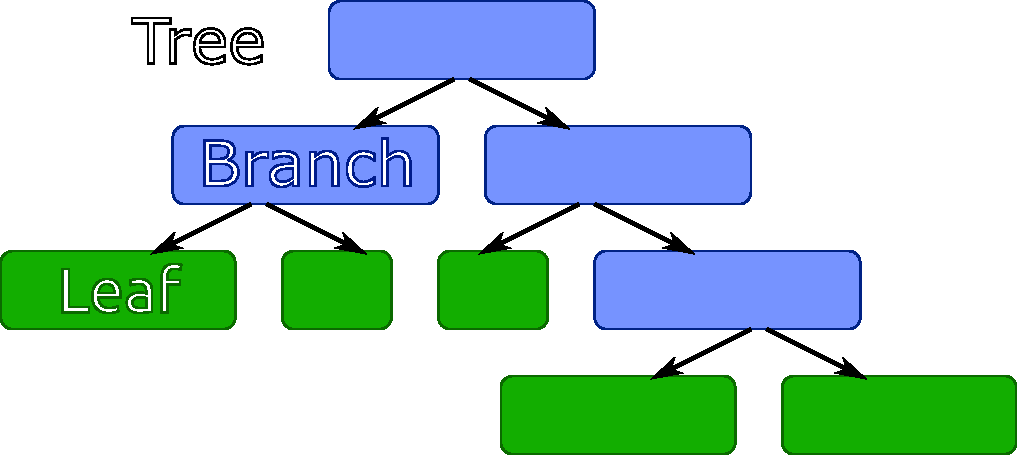
\includegraphics[width=0.5\linewidth]{images/boost/tree_scheme.pdf}
    \caption{One desicion tree - weak learner.}
    \label{fig:tree_scheme}
\end{figure}


Decision trees are a class of algorithms employed for both classification and regression tasks. They have gained popularity due to their ease of interpretation and resemblance to human decision-making processes~\cite{kotsiantis2013decision, song2015decision}. The methodology behind decision trees involves creating a tree-like model (see Fig.~\ref{fig:tree_scheme}) of decisions based on the values of input features, which is particularly effective for data mining applications~\cite{song2015decision}. 
One of the notable advancements in decision tree algorithms came with Ross Quinlan's development of ID3 and its improved version C4.5, which extended the capability to handle both categorical and numerical features through the use of 
% information gain ratio (IGR) 
\acrfull{igr} (see~\cite{mienye2019prediction} for information).


Building upon the foundation laid by decision trees, ensemble learning techniques like 
% Random Forests (RF)
\acrfull{rf}
and \acrfull{gb} have been developed to tackle more complex problems. \acrlong{rf}s extend the decision tree concept by constructing a 'forest' of decision trees, each trained on a random subset of the data and features. The ensemble's final prediction is an aggregation of the predictions from individual trees, significantly reducing variance compared to a single decision tree, and often achieving higher accuracy.

\begin{figure}[ht]
   \centering
    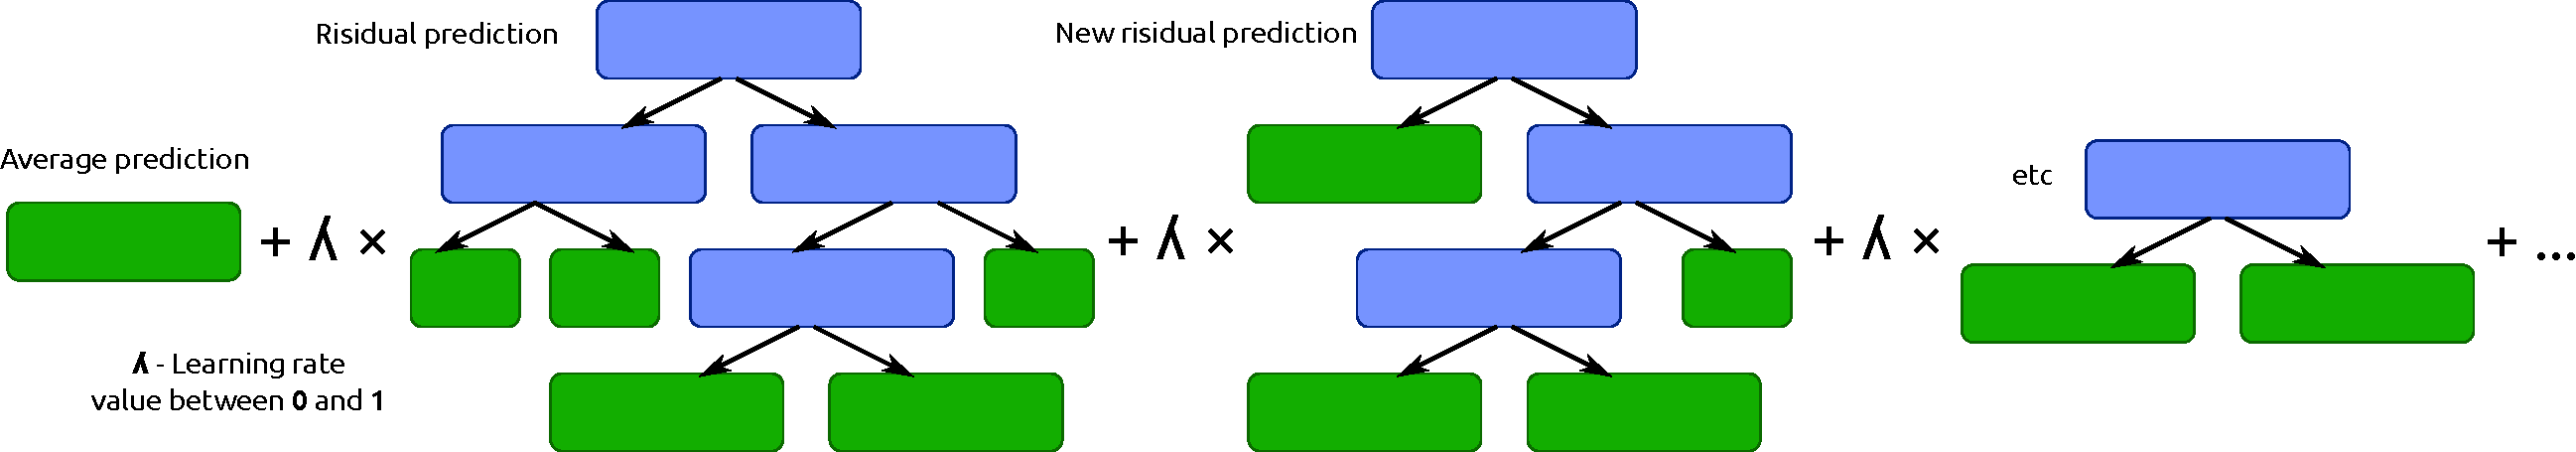
\includegraphics[width=1\linewidth]{images/boost/boosting_scheme.pdf}
    \caption{Gradient boosting scheme}
    \label{fig:boosting_scheme}
\end{figure}

On the other hand, \acrlong{gb} takes a sequential approach to ensemble learning. Unlike \acrlong{rf}s, which build trees independently, \acrlong{gb} iteratively trains decision trees to correct the errors of their predecessors, as depicted in Fig.~\ref{fig:boosting_scheme}. By minimizing a loss function through a gradient descent-like optimization, \acrlong{gb} gradually improves the accuracy of its predictions. This iterative correction process enables \acrlong{gb} to adapt more effectively to the data, often outperforming other tree-based ensemble methods like \acrlong{rf}s in terms of predictive accuracy~\cite{natekin2013gradient}. Variants like XGBoost, LightGBM, and CatBoost have emerged, focusing on enhancing speed and accuracy of this ensemble technique~\cite{bentejac2021comparative}.

% \subsubsection{Gradient Boosting in Optical Communication Systems}

\acrlong{gb} has garnered attention as a promising equalization technique for optical communication systems due to its adaptability and capability to model complex input-output relationships \cite{Chen:2016:XST:2939672.2939785,natekin2013gradient,friedman2002stochastic,bentejac2021comparative}. One of its notable advantages is its robustness to overfitting, achieved through techniques like shrinkage, regularization, and early stopping. Furthermore, the inherent parallelizability of \acrlong{gb} allows for efficient implementations on modern hardware architectures, including multi-core \acrshort{cpu}s, \acrshort{gpu}s, and even \acrshort{fpga}s \cite{alcolea2021fpga}, thus offering low-latency and power-efficient solutions crucial for real-time applications in optical communication systems.

In this part, we delve into the application of
% Gradient Boosting
\acrshort{gb}
as a novel equalization technique in optical communication systems. We aim to explore its potential to surpass the performance of traditional equalization methods, focusing on increasing predictive performance while simultaneously reducing the computational complexity of the equalization process. This innovative approach positions \acrlong{gb} as a promising candidate for equalization tasks in optical communication systems, opening avenues for future advancements in the field.

\subsection{Regression Trees Foundations}
Decision Trees enable the modeling of outcomes based on decision rules inferred from data attributes. While decision trees can be applied for both classification and regression tasks, this work focuses on their use in regression, aiming to predict continuous outcomes.

The operation of regression trees relies on mathematical concepts to split the data at each node in a way that results in subsets with minimized variance. 
Variance measures the spread of a dataset's values. It is defined as:
\begin{equation}
    \mathrm{Var}(Y) = \frac{1}{N} \sum_{i=1}^{N} (y_i - \bar{y})^2
\end{equation}
where $Y$ is the set of target values, $y_i$ is an individual target value, $\bar{y}$ is the mean of the target values, and $N$ is the number of data points.

When selecting the best feature to split on at each node, the decision tree algorithm seeks to maximize the reduction in variance. This is defined as the difference between the variance before the split and the weighted average variance of the two child nodes after the split:
\begin{equation}
    \mathrm{Var}_{reduction} = \mathrm{Var}(\mathrm{parent}) - \left( \frac{N_{left}}{N} \mathrm{Var}(\mathrm{left}) + \frac{N_{right}}{N} \mathrm{Var}(\mathrm{right}) \right)
\end{equation}
Maximizing this reduction ensures that the resulting child nodes are as homogenous as possible.
Mean Squared Error is another measure used to evaluate the performance of a regression tree, particularly for leaf nodes. It is defined as:
\begin{equation}
    \mathrm{MSE} = \frac{1}{N} \sum_{i=1}^{N} (y_i - \hat{y})^2
\end{equation}
where $\hat{y}$ is the predicted value for the data points in the leaf node, typically the mean of the target values of the data points in the node.


\begin{enumerate}
    \item \textbf{Start at the Root:} The entire dataset is considered at the root node.
    \item \textbf{Feature Selection for Splitting:} The algorithm evaluates each possible split across all features, calculating the variance for the dataset if it were split according to each feature. The reduction in variance for each potential split is determined by comparing the total variance before the split with the weighted sum of the variances of the two resulting subsets. At each node, select the feature that, when split upon, results in child nodes with the lowest total variance.
    \item \textbf{Splitting the Data:} The dataset is split into subsets based on the selected feature's values, creating child nodes.
    \item \textbf{Recursive Partitioning:} Repeat the feature selection and splitting process recursively on each child node until stopping criteria are met, such as a maximum tree depth or a minimum number of samples in a node.
    \item \textbf{Leaf Nodes and Prediction:} Each leaf node represents a numerical value, typically the mean of the target values in the node. This value is the prediction for new instances that reach this leaf.
    \item \textbf{Predicting New Instances:} To predict a new instance, traverse the tree from the root, following the branches based on the instance's features, until a leaf node is reached. The value of the leaf node is the predicted outcome.
\end{enumerate}

This approach ensures that the tree is constructed in a way that captures the underlying patterns in the data as efficiently as possible.

% \begin{algorithm}
% \caption{Decision Tree Algorithm}
% \label{alg:tree}
% \begin{algorithmic}[1]
% \State $\text{Start with the root node, containing all samples}$
% \While{$\text{termination criteria not met}$}
%     \For{$\text{each feature}$}
%         \For{$\text{each possible split}$}
%             \State {$\text{Calculate the impurity decrease}$}
%         \EndFor
%         \State {$\text{Choose the split that maximizes the impurity decrease}$}
%     \EndFor
%     \State $\text{Split the node into two child nodes}$
%     \State $\text{Assign each sample to a child node}$
%     \If{$\text{termination condition of a node is met}$}
%         \State $\text{Mark it as a leaf and assign it a prediction}$
%     \EndIf
% \EndWhile
% \end{algorithmic}
% \end{algorithm}

\subsection{Theory of Gradient Boosting}

\acrfull{gb} builds a series of weak learners, usually decision trees, and iteratively refines the model by focusing on the areas where the previous models performed poorly. 
The algorithm starts with an initial model, \( F_0(x) \), which could be as simple as predicting the mean (for regression) or the majority class (for classification) for all instances in the dataset.

\begin{equation}
    F_0(x) = \arg\min_{\gamma} \sum_{i=1}^N L(y_i, \gamma) {,}
\end{equation}
where: \( N \) is the number of training instances,
\( L \) is the loss function,
\( y_i \) is the true label of the \( i \)-th instance,
\( \gamma \) is a constant.

In classification tasks, the concept of a ``majority class,'' which denotes the most frequently occurring class in the dataset, is often employed as the starting point for initializing models in algorithms like gradient boosting. This initial model, \(F_0(x)\), uniformly predicts the majority class for all instances, providing a baseline from which the algorithm can iteratively improve. However, this approach encounters difficulties in applications like 16-\acrshort{qam} constellation point prediction, where classes (i.e., constellation points) are nearly equally represented, and thus, no single class dominates. In such cases, selecting a class at random for \(F_0(x)\) might serve as an unbiased alternative, ensuring a simple yet effective starting point for model refinement. This adaptation underscores the necessity for flexible initial modeling strategies in the face of varied data distributions, particularly in complex classification scenarios.

The algorithm then enters a loop, for \( m = 1 \) to \( M \) (where \( M \) is the number of boosting rounds), where in each round it:
\begin{enumerate}
    \item Computes the pseudo-residuals, which are the gradients of the loss function with respect to the predicted values of the previous model, \( F_{m-1}(x) \):

\begin{equation}
r_{im} = -\left[\frac{\partial L(y_i, F(x_i))}{\partial F(x_i)}\right]_{F(x)=F_{m-1}(x)}
\end{equation}

    \item Fits a weak learner, \( h_m(x) \), to the pseudo-residuals, \( r_{im} \).

    \item Computes the optimal step size, \( \alpha_m \), that minimizes the loss function when \( h_m(x) \) is added to the current model:

\begin{equation}
\alpha_m = \arg\min_{\alpha} \sum_{i=1}^N L(y_i, F_{m-1}(x_i) + \alpha h_m(x_i))
\end{equation}

    \item Updates the model:

\begin{equation}
F_m(x) = F_{m-1}(x) + \alpha_m h_m(x)
\end{equation}

\end{enumerate}

The final model is the sum of the initial model and the products of the step sizes and the weak learners from each round:

\begin{equation}
F_M(x) = F_0(x) + \sum_{m=1}^M \alpha_m h_m(x)
\end{equation}


Each weak learner, \( h_m(x) \), is typically a shallow decision tree, and the loss function, \( L \), could be any differentiable loss function such as Mean Squared Error for regression or Logarithmic Loss for classification. The step size, \( \alpha_m \), helps in controlling the contribution of each weak learner, aiding in reducing overfitting and improving the model's generalization capability.

\subsubsection{Loss Functions}

Loss functions measure the difference between the predicted values and the true values. In \acrlong{gb}, differentiable loss functions are used. The two common ones are \Gls{mse} (for regression) and Logistic Loss (for binary classification).

The loss function for \gls{mse} is given by:
\begin{equation}
L(y, F(x)) = \frac{1}{N} \sum_{i=1}^N (y_i - F(x_i))^2
\end{equation}

Taking the derivative with respect to \( F(x_i) \), we get:
\begin{equation}
\frac{\partial L(y, F(x))}{\partial F(x_i)} = -2(y_i - F(x_i))
\end{equation}

The loss function for Logistic Loss is given by:
\begin{equation}
L(y, F(x)) = - \frac{1}{N} \sum_{i=1}^N [ y_i \log(F(x_i)) + (1-y_i) \log(1-F(x_i)) ]
\end{equation}

Taking the derivative with respect to \( F(x_i) \), we get:
\begin{equation}
\frac{\partial L(y, F(x))}{\partial F(x_i)} = \frac{F(x_i) - y_i}{F(x_i)(1 - F(x_i))}
\end{equation}

In these formulas: \( N \) is the number of samples, \( y_i \) is the true label of the \( i \)-th instance, \( F(x_i) \) is the predicted value for the \( i \)-th instance.

For \gls{mse}, the derivative is straightforward and results in a simple expression involving the difference between the actual and predicted values.
For Logistic Loss, the derivative involves the quotient rule, and the expression relates the difference between the predicted probability and the actual label, normalized by the product of the predicted probability and its complement.


\subsubsection{Regularization}

Regularization is a technique used to prevent overfitting by adding a penalty on the complexity of the model. In \acrlong{gb}, regularization can be achieved through various means:

\begin{enumerate}
    \item \textbf{Shrinkage (Learning Rate)}: 
    A small learning rate (also known as shrinkage) can be used to reduce the step size at each boosting step, making the boosting process more conservative.
    \[ F_m(x) = F_{m-1}(x) + \nu \cdot \alpha_m h_m(x) \]
    where \( \nu \) is the learning rate, \( 0 < \nu \leq 1 \).

    \item \textbf{Tree Complexity}:
    The complexity of the individual trees can be controlled by setting a maximum depth, minimum samples per leaf, or other similar parameters.

    \item \textbf{L1 (Lasso) and L2 (Ridge) Regularization}:
    These regularization terms can be added to the loss function to penalize the coefficients of the features.
    \[ L_{\text{regularized}}(y, F(x)) = L(y, F(x)) + \lambda_1 \sum | \beta | + \lambda_2 \sum \beta^2 \]
    where \( \beta \) are the coefficients of the features, and \( \lambda_1 \) and \( \lambda_2 \) are the regularization parameters.
\end{enumerate}


\subsection{Methodology}


In this study, we introduce a novel approach to nonlinear equalization in optical communication systems by employing a \acrshort{gb} algorithm based on decision trees.
We used an optical channel model of \acrfull{ssmf} with \acrlong{edfa}s (\acrshort{edfa}s). The signal format is a 16-quadrature amplitude modulation (16-\acrshort{qam}) WDM with dual polarization and a symbol rate of $34.4\;\textrm{GBd}$. The pulse shaping employed a digital \acrfull{rrc} filter with a roll-off factor of $0.1$. The transmission distance varied between $10$, $15$, and $20$ spans of $80\;\textrm{km}$ each. The \acrshort{edfa} noise figure was set at $4.5\;\textrm{dB}$. The average signal power range was from $1$ to $8\;\textrm{dBm}$, but for training, we used power from $4\;\textrm{dBm}$ to $8 \textrm{dBm}$. The signal propagation through the fiber was represented by a generalized Manakov equation using the \acrshort{gpu}-accelerated split-step Fourier method\cite{esf0_2023_7880552}. The fiber parameters included a wavelength of $\lambda = 1550\;\textrm{nm}$, a dispersion coefficient of $D = 16.8\;\textrm{ps}/(\textrm{nm} \cdot \textrm{km})$, and a nonlinear coefficient of $\gamma = 1.2\;\textrm{W}^{-1} \cdot \textrm{km}^{-1}$.


We generated around $10$ million datapoints for each specific average power and propagation distance. The dataset was then divided into training and test sets, with the test set comprising $1\%$ of the full dataset (about $100,000$ points).

In the dataset used for training, the input consists of values of the received points for the x-polarization, for which we aim to predict the nonlinear shift. To account for the neighboring points' influence, we include five values of received points to the right and left of the central point (neighbors in the sequence of points). Since we utilize two polarizations, we also incorporate the central point for y-polarization (in the same position in the sequence as for x-polarization) and its five neighboring points on both the left and right. As a result, a total of 22 complex points serve as input for the \acrshort{gb} algorithm. The output represents the nonlinear shift (a complex number that must be added to accurately shift the point to its original position in the constellation) for the received point in the x-polarization.

The gradient boosting algorithm was implemented using the XGBoost library\cite{Chen:2016:XST:2939672.2939785} with \acrshort{gpu} acceleration. The training process involved a large number of estimators, specifically $200,000$, which were chosen to test the idea of using decision trees but can be significantly reduced for a particular system. The maximum tree depth did not exceed $20$, the learning rate was set to $0.1$, and the $L_2$ and $L_1$ regularization parameters were both set to $1.0$.

To explore why we limited our analysis to only five neighboring symbols, despite the potential for dispersion broadening to impact a significantly larger number of symbols (thus, with nonlinear effects, the effective interaction could extend to dozens or hundreds of symbols), let us provide some context to support this decision.

Machine learning models, with their capacity to serve as universal approximators, can extract valuable information from input data for a specific purpose. This introduction sets the stage for our specific scenario: the presence of neighboring points, which are themselves influenced by their neighbors. This implies that the nonlinear adjustment of neighbors, even with knowledge only of a neighbor's position at the receiver, can reveal information about subsequent neighbors and the influence on the target point for which we are calculating a correction. This forms a complex network where information about a local group of points contains more insights than initially considered. For instance, the outermost points in our analysis (the fifth neighbors to the left and right) indirectly incorporate information about subsequent points in the transmitted sequence. This information is partial but suggests that each point's shift due to neighboring influences carries implicit data. Although expanding the number of neighbor symbols for analysis could potentially enhance model performance, such an exploration exceeds the scope of this research. However, we emphasize that this is a compelling and valuable area for future investigation and would be an excellent subject for a detailed study.

Now, let's turn our attention to a more quantitative analysis. We will examine how features (the neighboring points) are utilized in a \acrlong{gb} model by employing feature importance measurement.


% \begin{figure}[tpb]
%     \begin{minipage}[h]{0.5\linewidth}
%     \center{
%         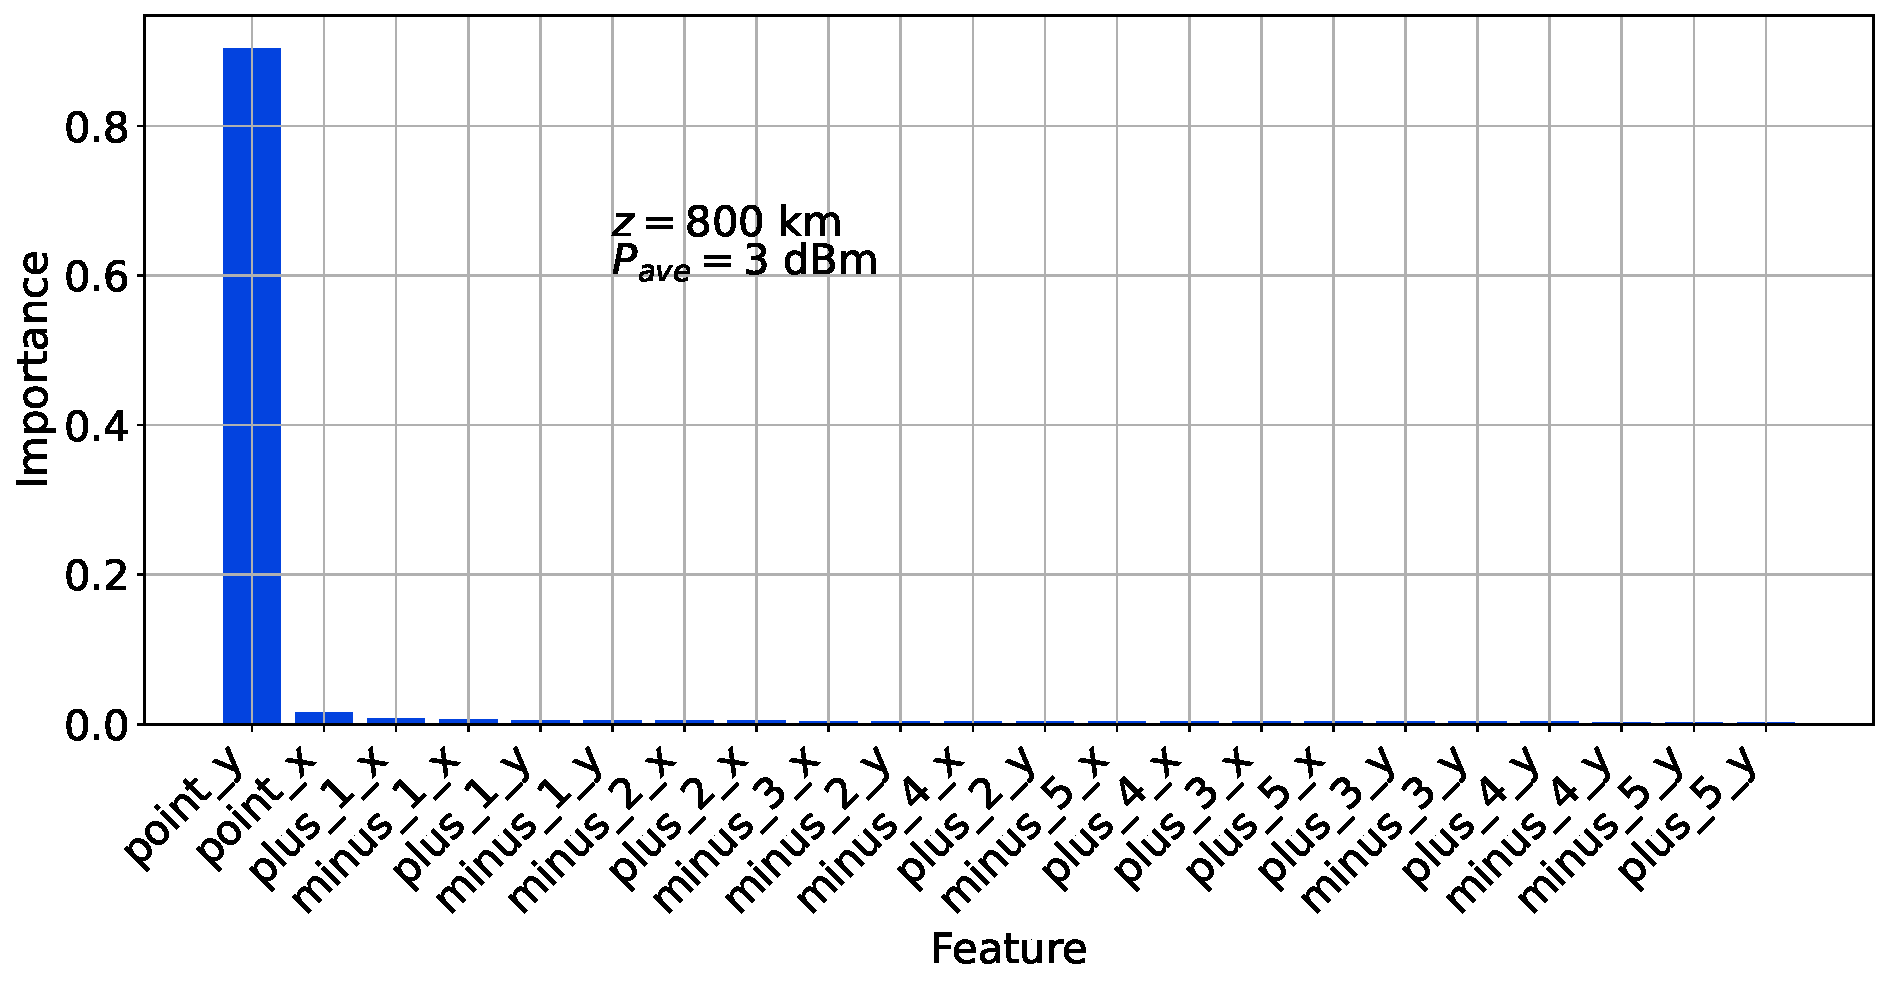
\includegraphics[width=1\linewidth]{images/boost/feature_importances_z800_pdbm3.pdf} (a)
%     }
%     \end{minipage}
%     \hfill
%     \begin{minipage}[h]{0.5\linewidth}
%     \center{
%         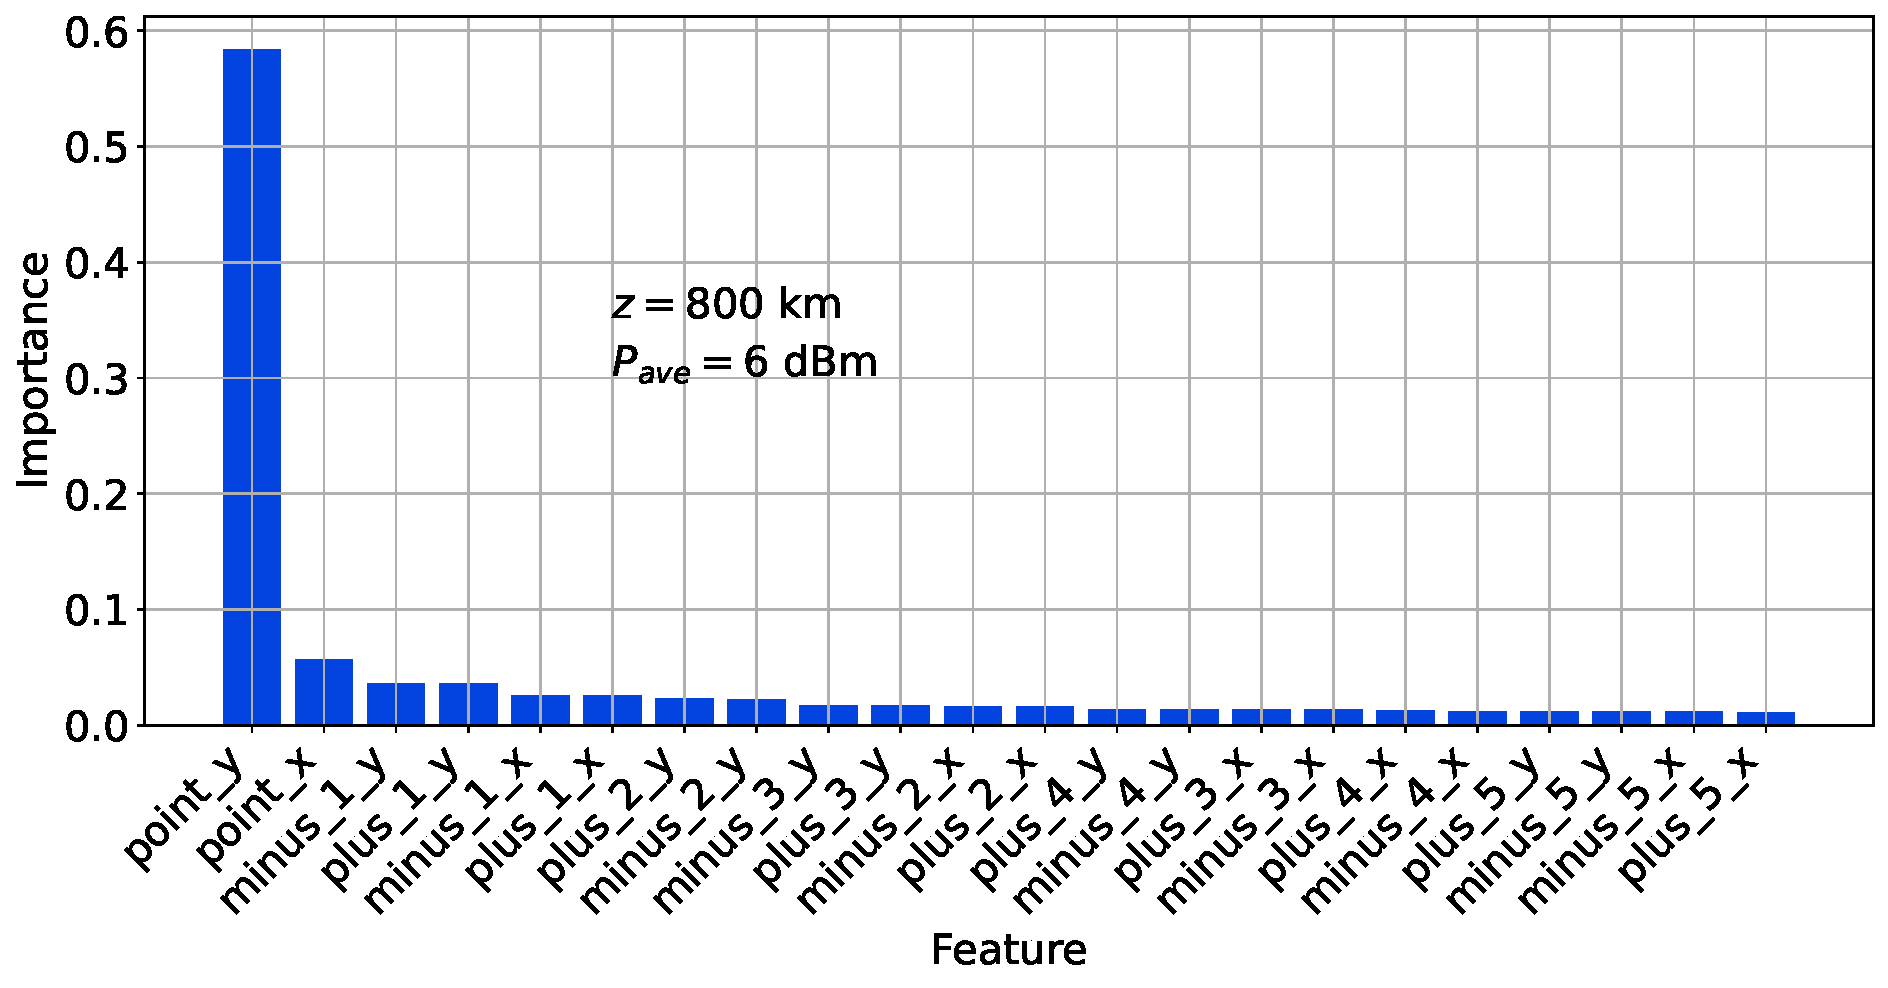
\includegraphics[width=1\linewidth]{images/boost/feature_importances_z800_pdbm6.pdf} (d)
%     }
%     \end{minipage}

%     \begin{minipage}[h]{0.5\linewidth}
%     \center{
%         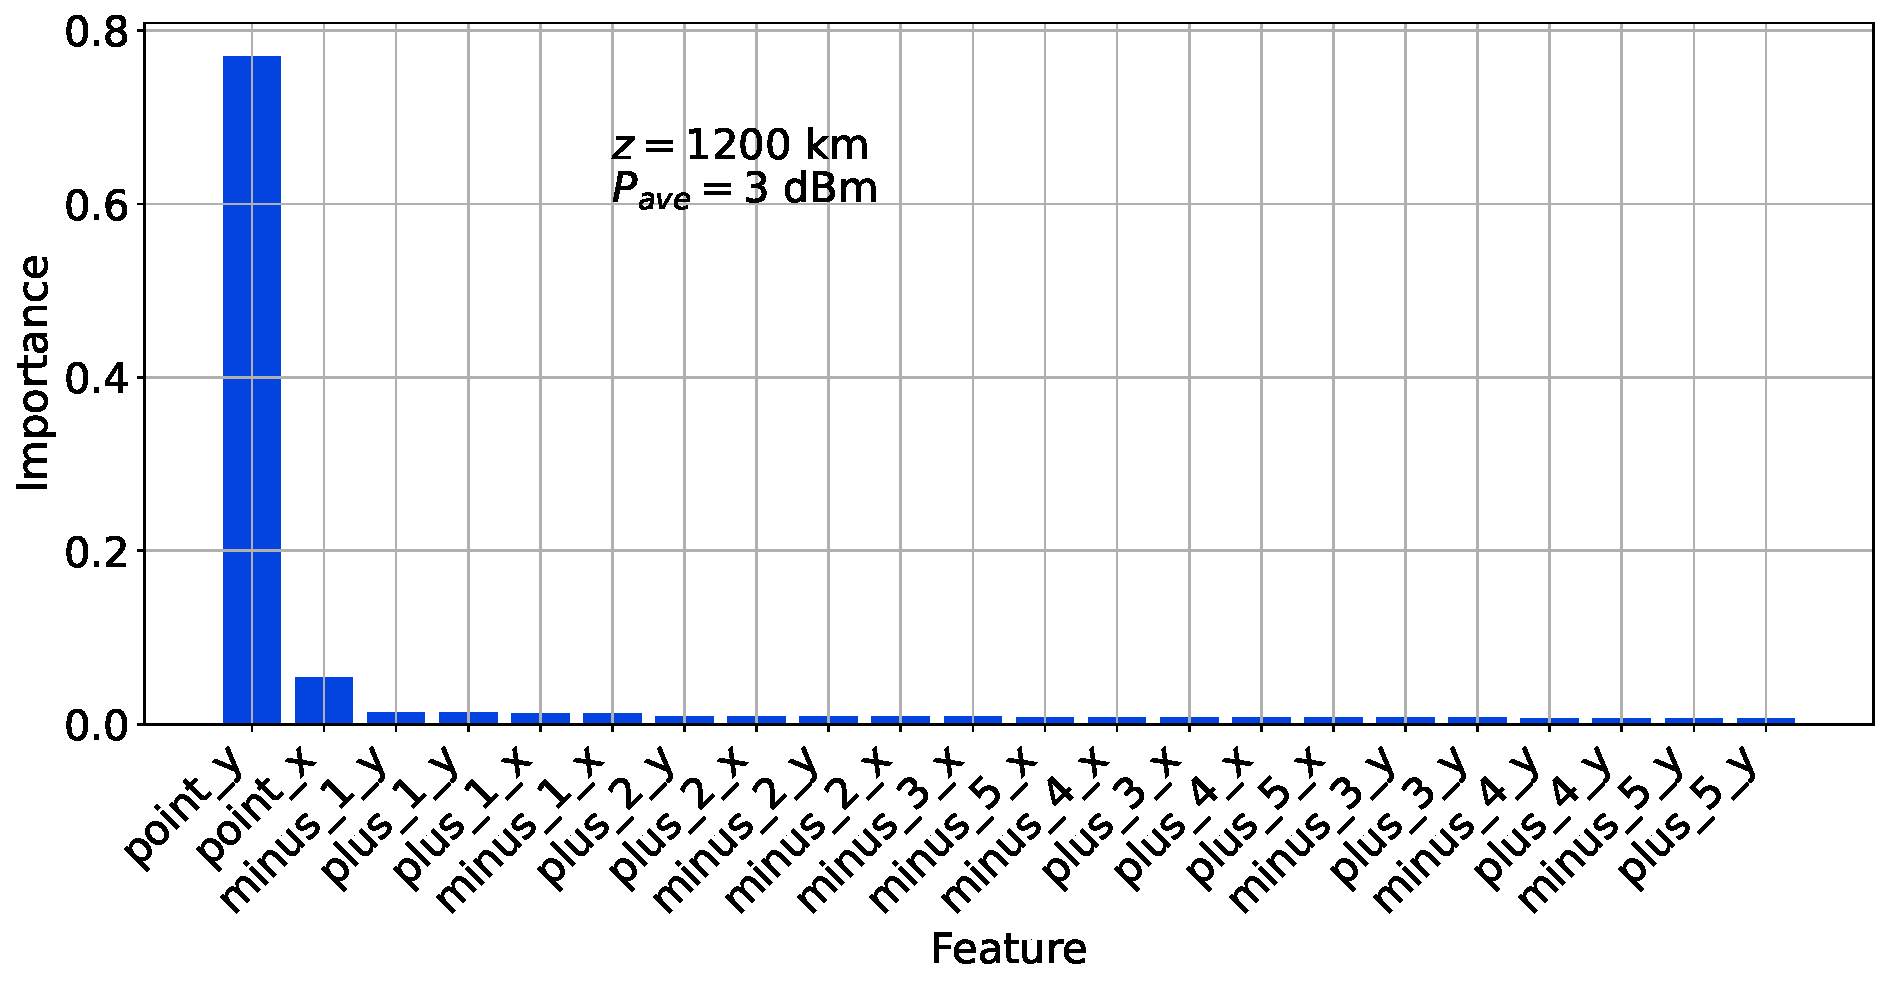
\includegraphics[width=1\linewidth]{images/boost/feature_importances_z1200_pdbm3.pdf} (b)
%     }
%     \end{minipage}
%     \hfill
%     \begin{minipage}[h]{0.5\linewidth}
%     \center{
%         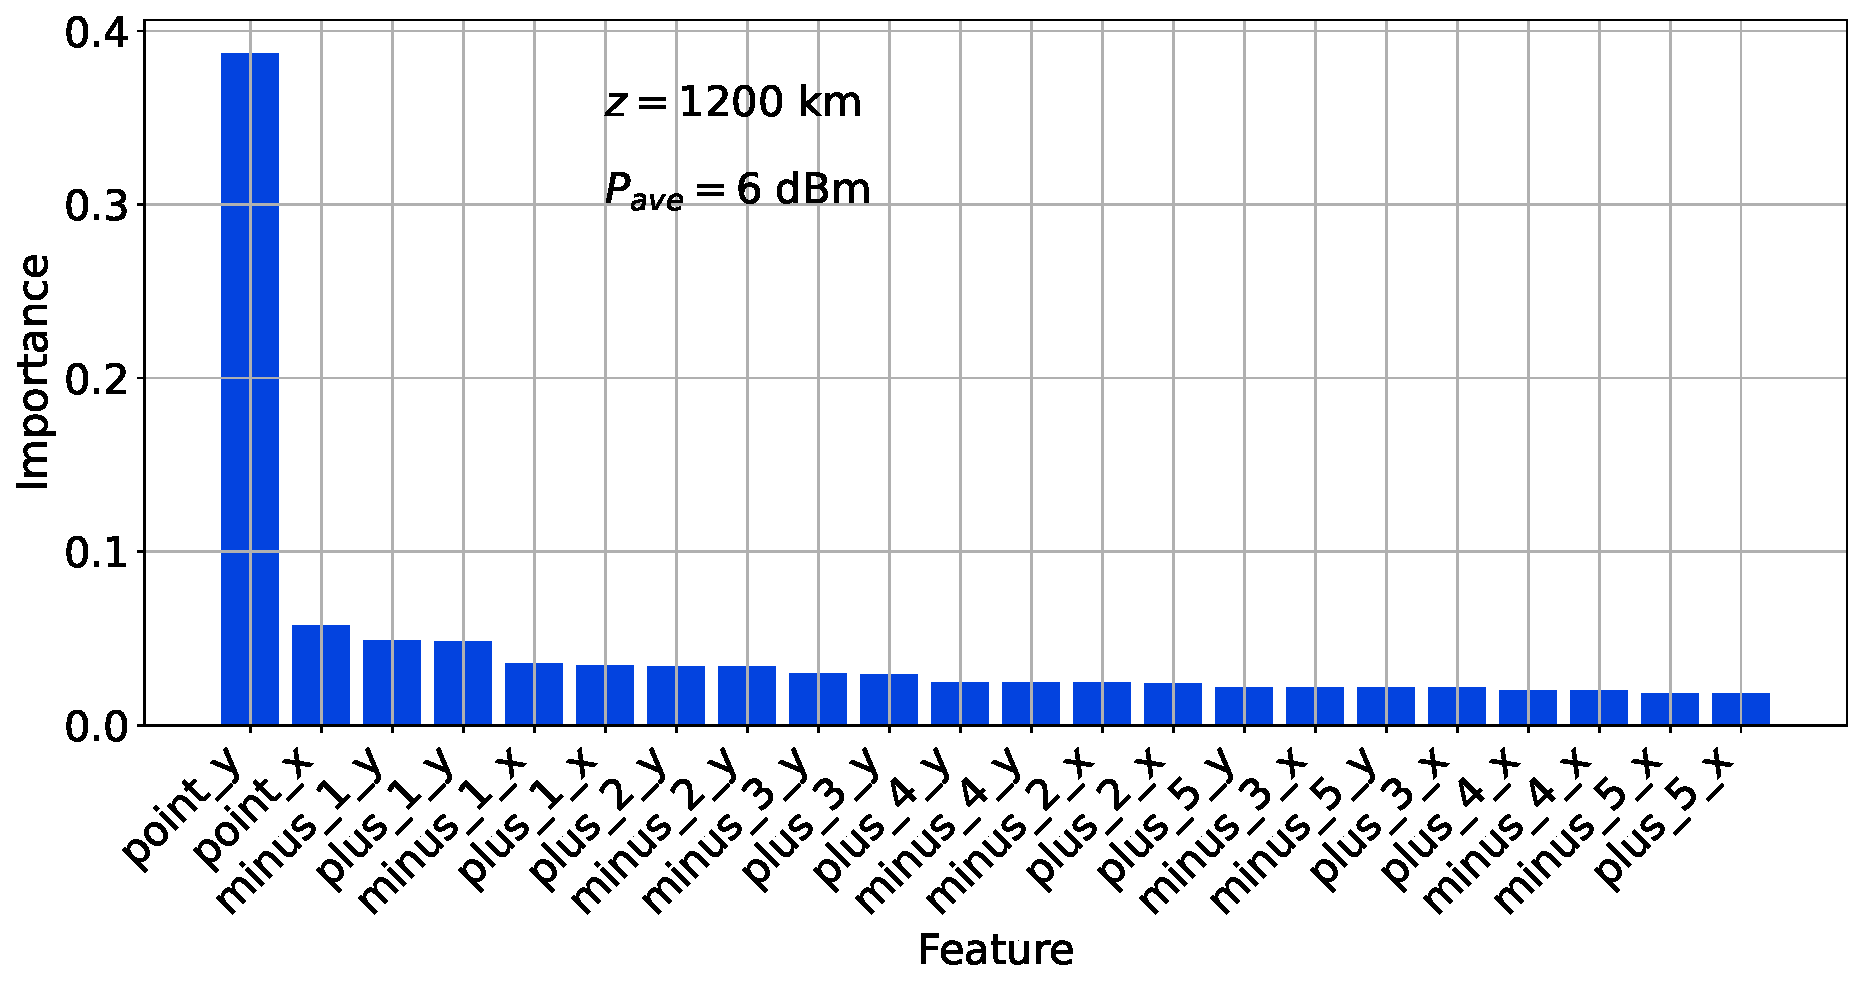
\includegraphics[width=1\linewidth]{images/boost/feature_importances_z1200_pdbm6.pdf} (e)
%     }
%     \end{minipage}

%     \begin{minipage}[h]{0.5\linewidth}
%     \center{
%         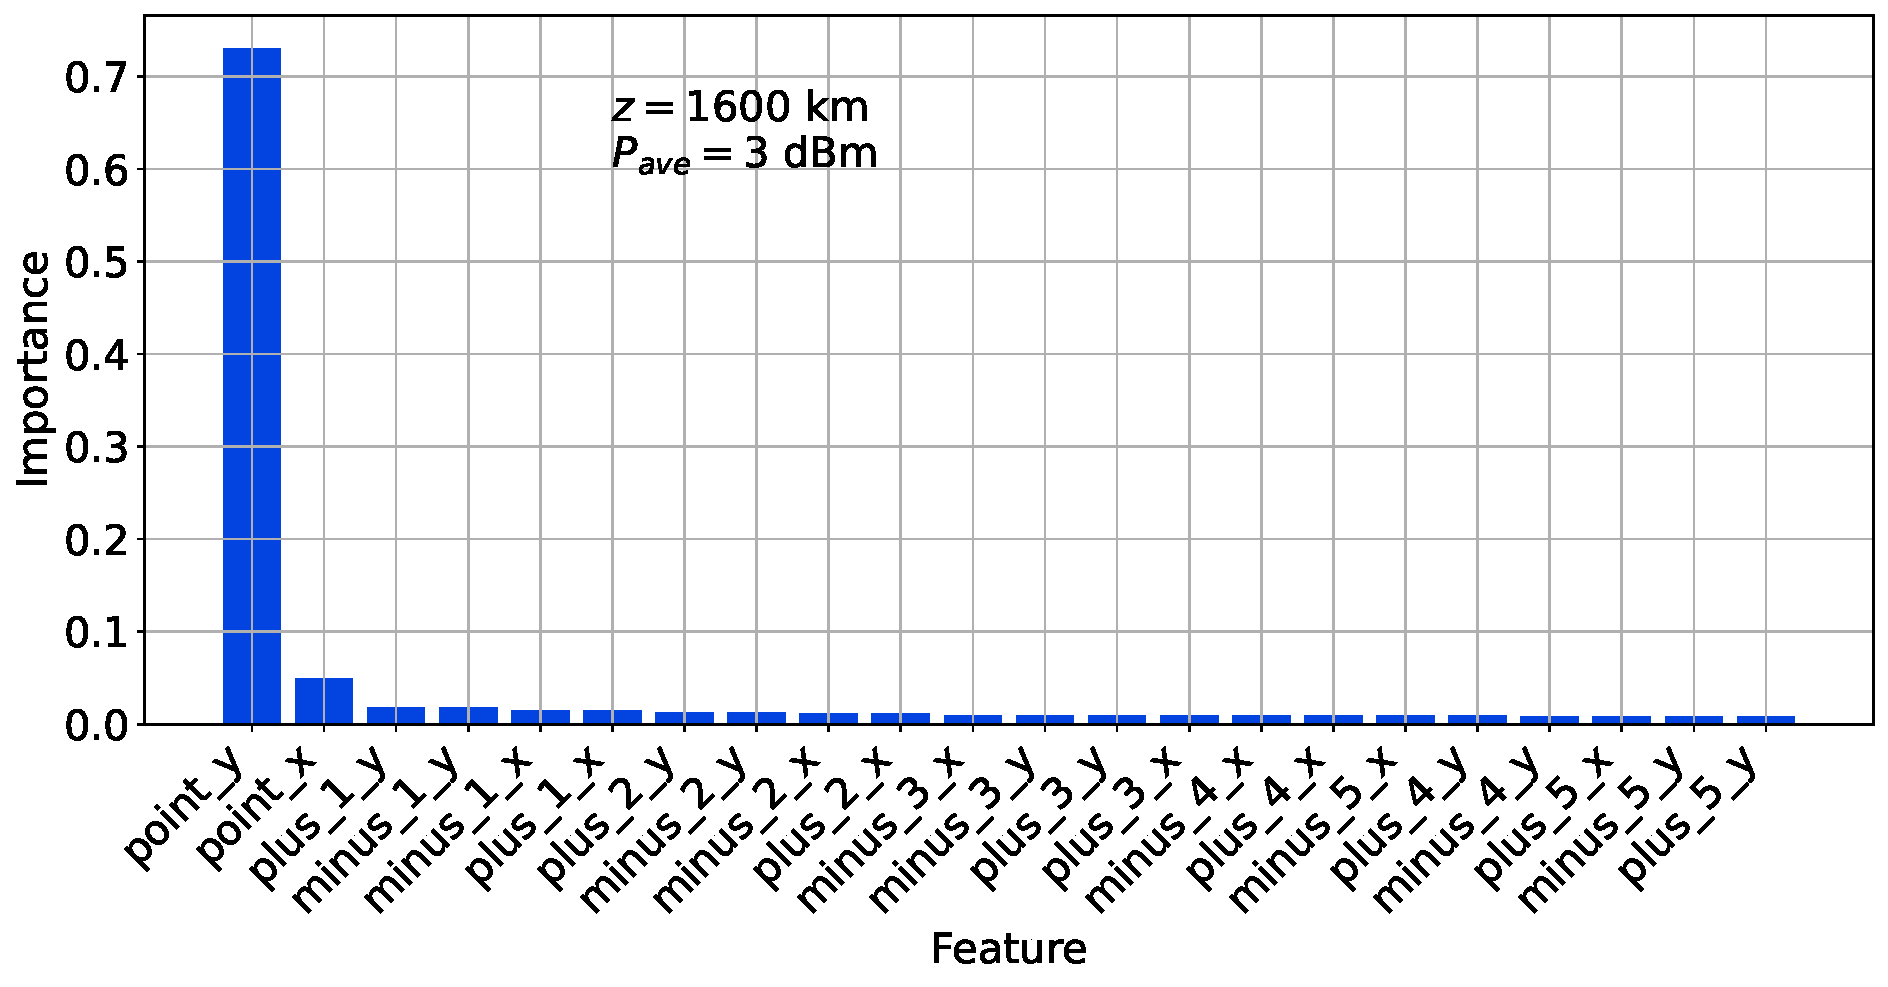
\includegraphics[width=1\linewidth]{images/boost/feature_importances_z1600_pdbm3.pdf} (c)
%     }
%     \end{minipage}
%     \hfill
%     \begin{minipage}[h]{0.5\linewidth}
%     \center{
%         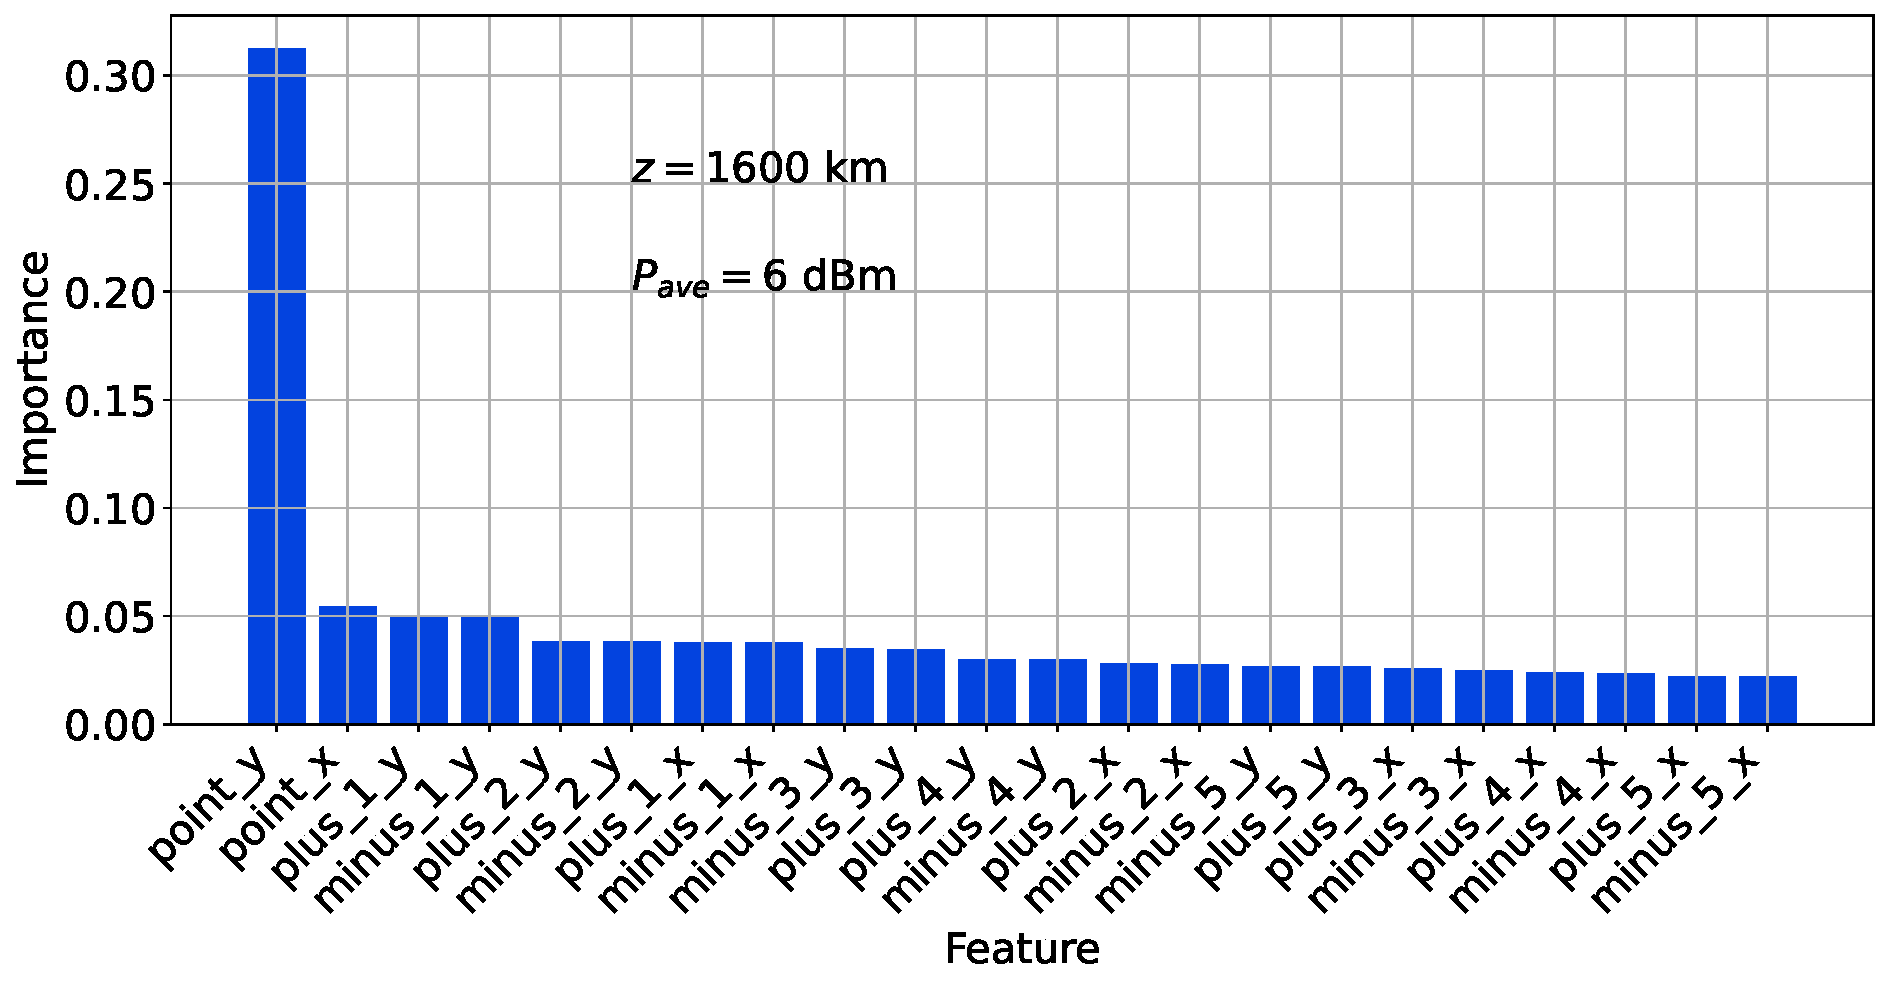
\includegraphics[width=1\linewidth]{images/boost/feature_importances_z1600_pdbm6.pdf} (f)
%     }
%     \end{minipage}
%     \caption{Examples of carrier functions for WDM signal. \textbf{(a)} function for Eq.~(\ref{eq:wdm_carrier}), \textbf{(b)} function for Eq.~(\ref{eq:wdm_carrier2}), \textbf{(c)} function for \gls{rc} (Eq.~(\ref{eq:rc_time})) and \textbf{(d)} for \gls{rrc} (Eq.~(\ref{eq:rc_time}).}
%     \label{fig:importance_gb}
% \end{figure}


\begin{figure}[tpb]
    \centering
    \begin{minipage}[h]{0.75\linewidth}
    \center{
        (a) 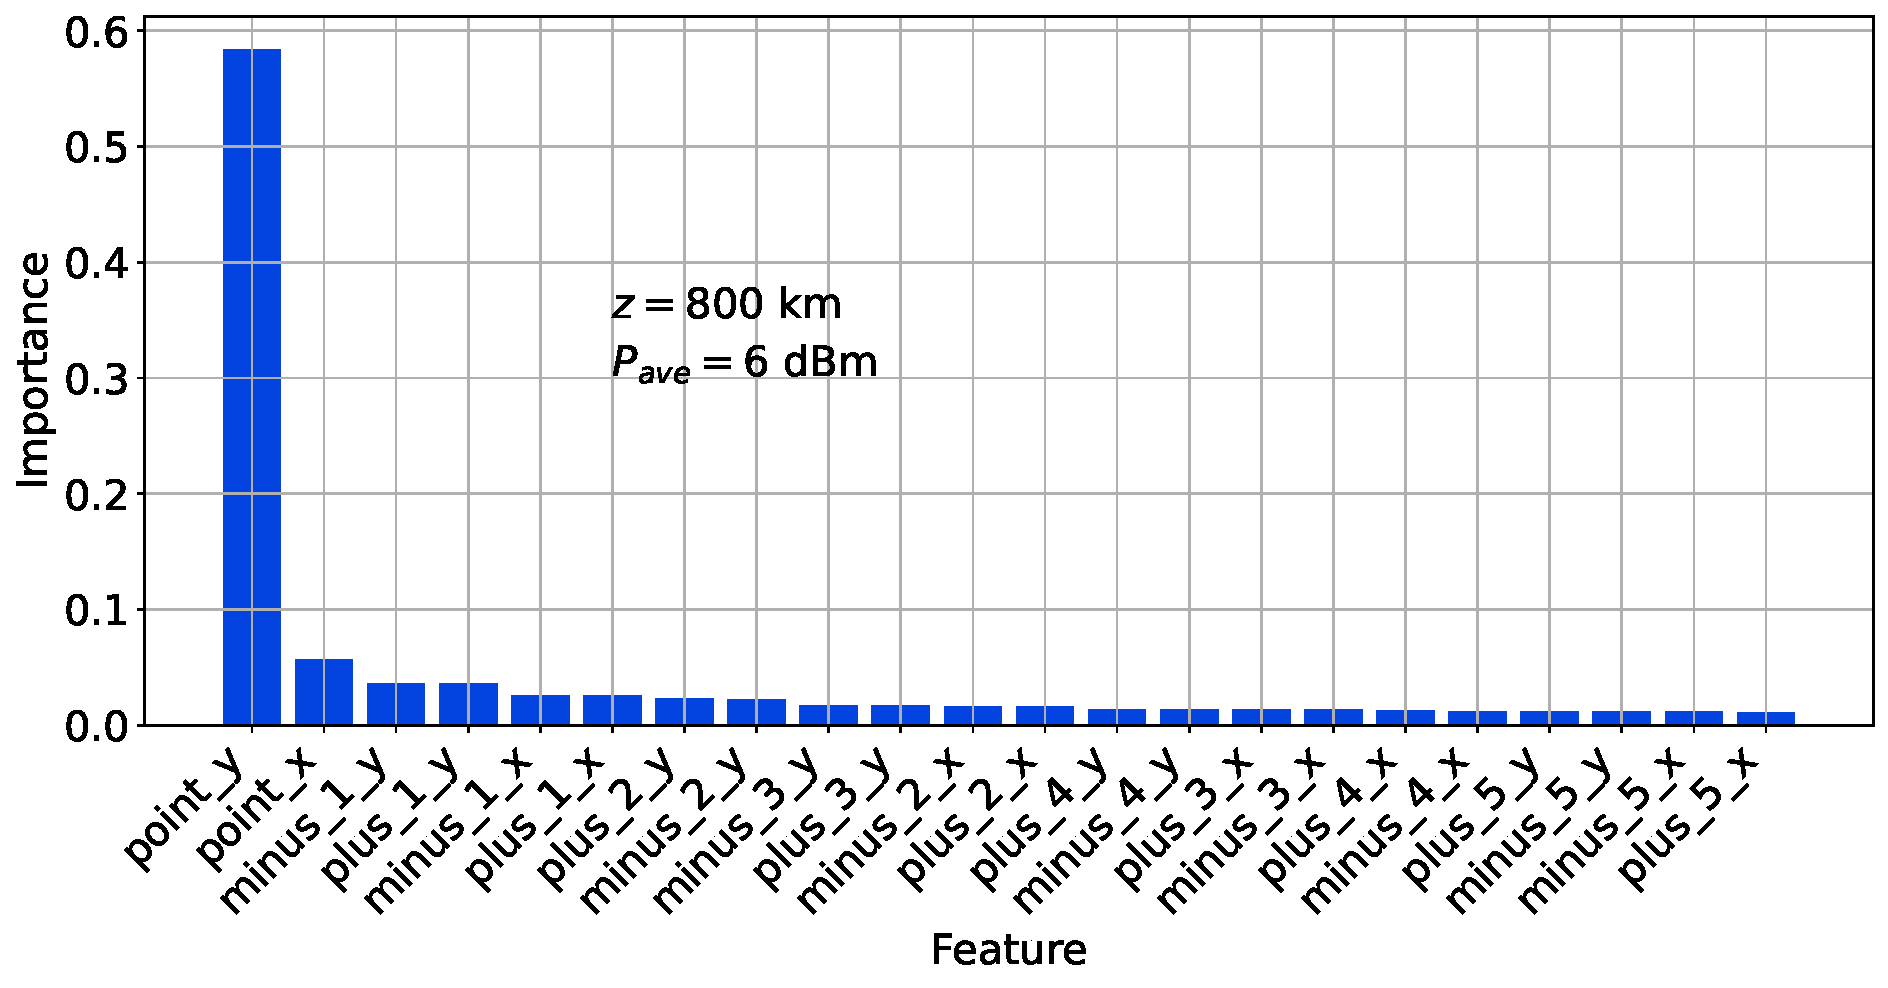
\includegraphics[width=1\linewidth]{images/boost/feature_importances_z800_pdbm6.pdf}
    }
    \end{minipage}

    \centering
    \begin{minipage}[h]{0.75\linewidth}
    \center{
        (b) 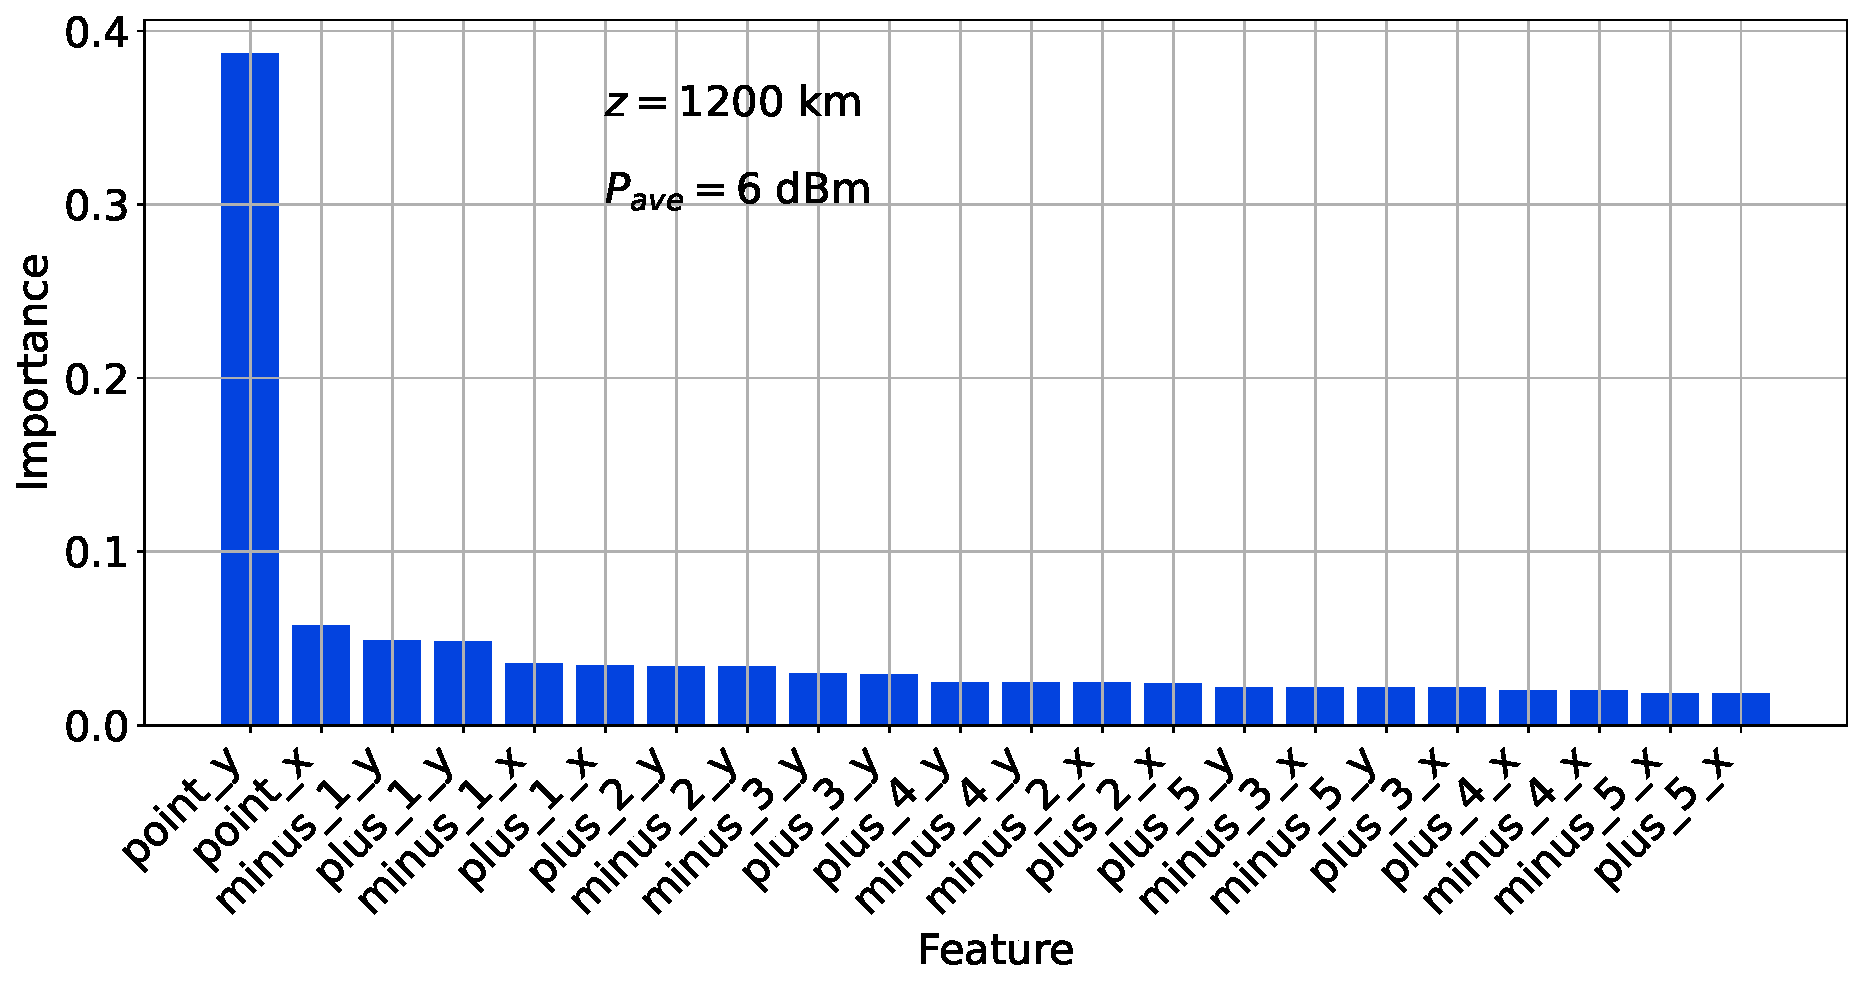
\includegraphics[width=1\linewidth]{images/boost/feature_importances_z1200_pdbm6.pdf}
    }
    \end{minipage}

    \centering
    \begin{minipage}[h]{0.75\linewidth}
    \center{
        (c) 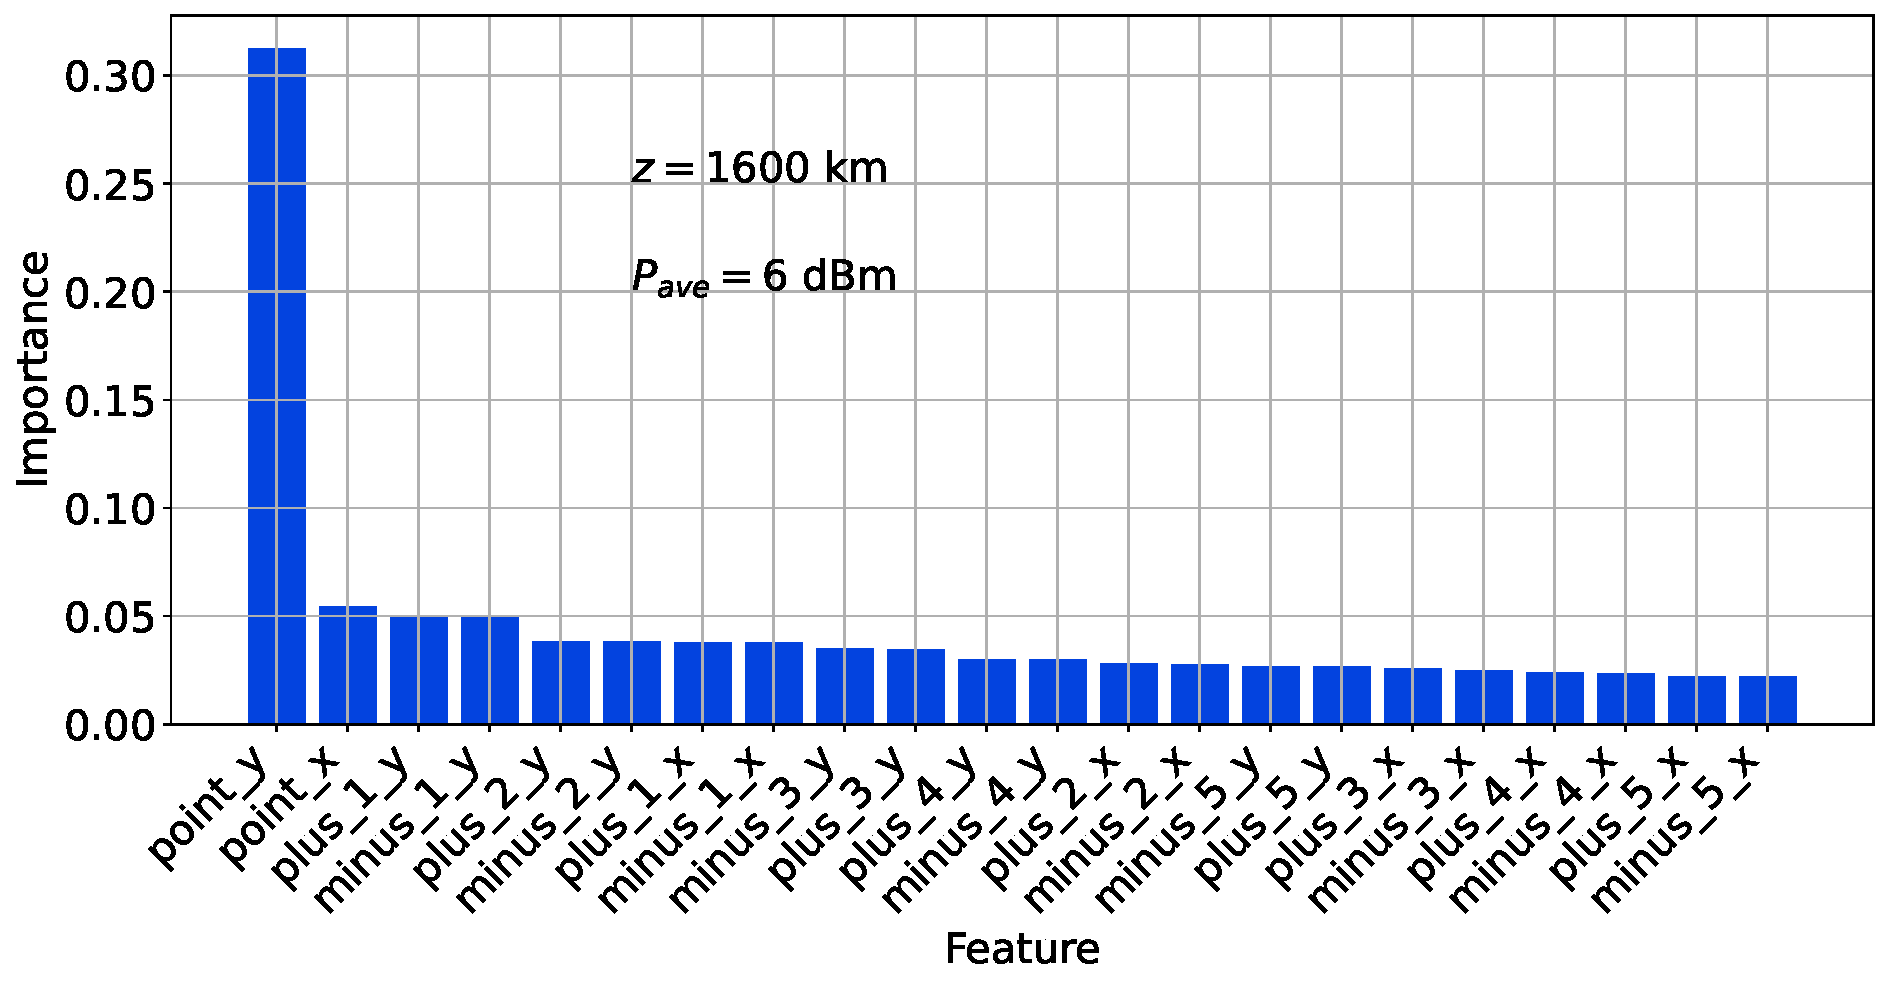
\includegraphics[width=1\linewidth]{images/boost/feature_importances_z1600_pdbm6.pdf}
    }
    \end{minipage}
    \caption{Feature importance in the trained \acrshort{gb} model for predicting nonlinear shifts at an average signal power of 6 dBm. \textbf{(a)} For a transmission distance of 800 km, \textbf{(b)} 1200 km, and \textbf{(c)} 1600 km. In the feature labels, `x' and `y' denote the polarization of the signal point, whereas `plus' and `minus' indicate the right and left neighbors in the symbol sequence, respectively.}
    \label{fig:importance_gb}
\end{figure}



Feature importance in gradient boosting models provides insight into the relative significance of each feature in making predictions. The importance of a feature is often quantified based on how frequently it is used to split the data across all trees in the ensemble. This metric, referred to as the "importance" or "weight," reflects the feature's contribution to the model's decision-making process.

Mathematically, we can define the importance of a feature as follows:
\begin{equation}
	I(f_i) = \frac{\sum_{k=1}^{K} \mathrm{Count}(f_i, T_k) }{\sum_{j=1}^{N} \sum_{k=1}^{K} \mathrm{Count}(f_j, T_k)} {,}
\end{equation}
where \(N\) represents the number of features, \(K\) the number of trees (estimators) in the model, and \(\mathrm{Count}(f_i, T_k)\) is the number of times feature \(f_i\) is used as a split in tree \(T_k\).

This definition implies that the importance of a feature is directly proportional to how often it is selected for splitting data points in the model's trees. A higher count indicates a higher significance of the feature in the model's predictions. The essence of this metric lies in its ability to highlight which features the model relies on most heavily to reduce uncertainty or entropy in the data.

It is essential to note that while this measure provides valuable insights into feature relevance, it does not convey the direction of the feature's effect (positive or negative) on the target variable. In the broader context of model interpretation and feature selection, understanding the importance of each feature helps in identifying the variables that contribute most significantly to the predictive power of the model. This knowledge can be crucial for model refinement, simplification, and for gaining deeper insights into the underlying processes being modeled.

Figure~\ref{fig:importance_gb} presents the feature importance in a \acrshort{gb} model trained to predict nonlinear shifts at an average signal power of 6 dBm for different transmission distances: (a) 800 km, (b) 1200 km, and (c) 1600 km. In the feature labels, `x' and `y' represent the polarization of the signal point, while 'plus' and 'minus' signify the right and left neighbors in the symbol sequence, respectively. An intriguing observation is that the most influential feature in the decision trees is not the point for which we predict the correction (`point\_x'), but its counterpart in the other polarization (`point\_y'). This finding highlights the significant insight that information from the same position but in a different polarization provides about the required correction.

Further analysis reveals that `point\_y' dominates feature usage, significantly more than `point\_x', especially over longer distances (for 1600 km, `point\_y' accounts for over 30\% of usage, whereas `point\_x' is just above 5\%). The importance of the immediate neighbors (`plus\_1\_y' and `minus\_1\_y') is comparable to `point\_x', but the relevance of further neighbors declines with their sequence number. This decline is more pronounced for shorter distances (800 km) compared to longer ones (1200 and 1600 km), aligning with the expectation that neighbor influence increases with distance. For instance, at 1600 km, the influence of the furthest neighbors analyzed is around 2\% each, dropping below 1\% for 1200 km, and to approximately 0.6\% for 800 km.

\begin{figure}[tpb]
    \centering
    \begin{minipage}[h]{0.75\linewidth}
    \center{
        (a) 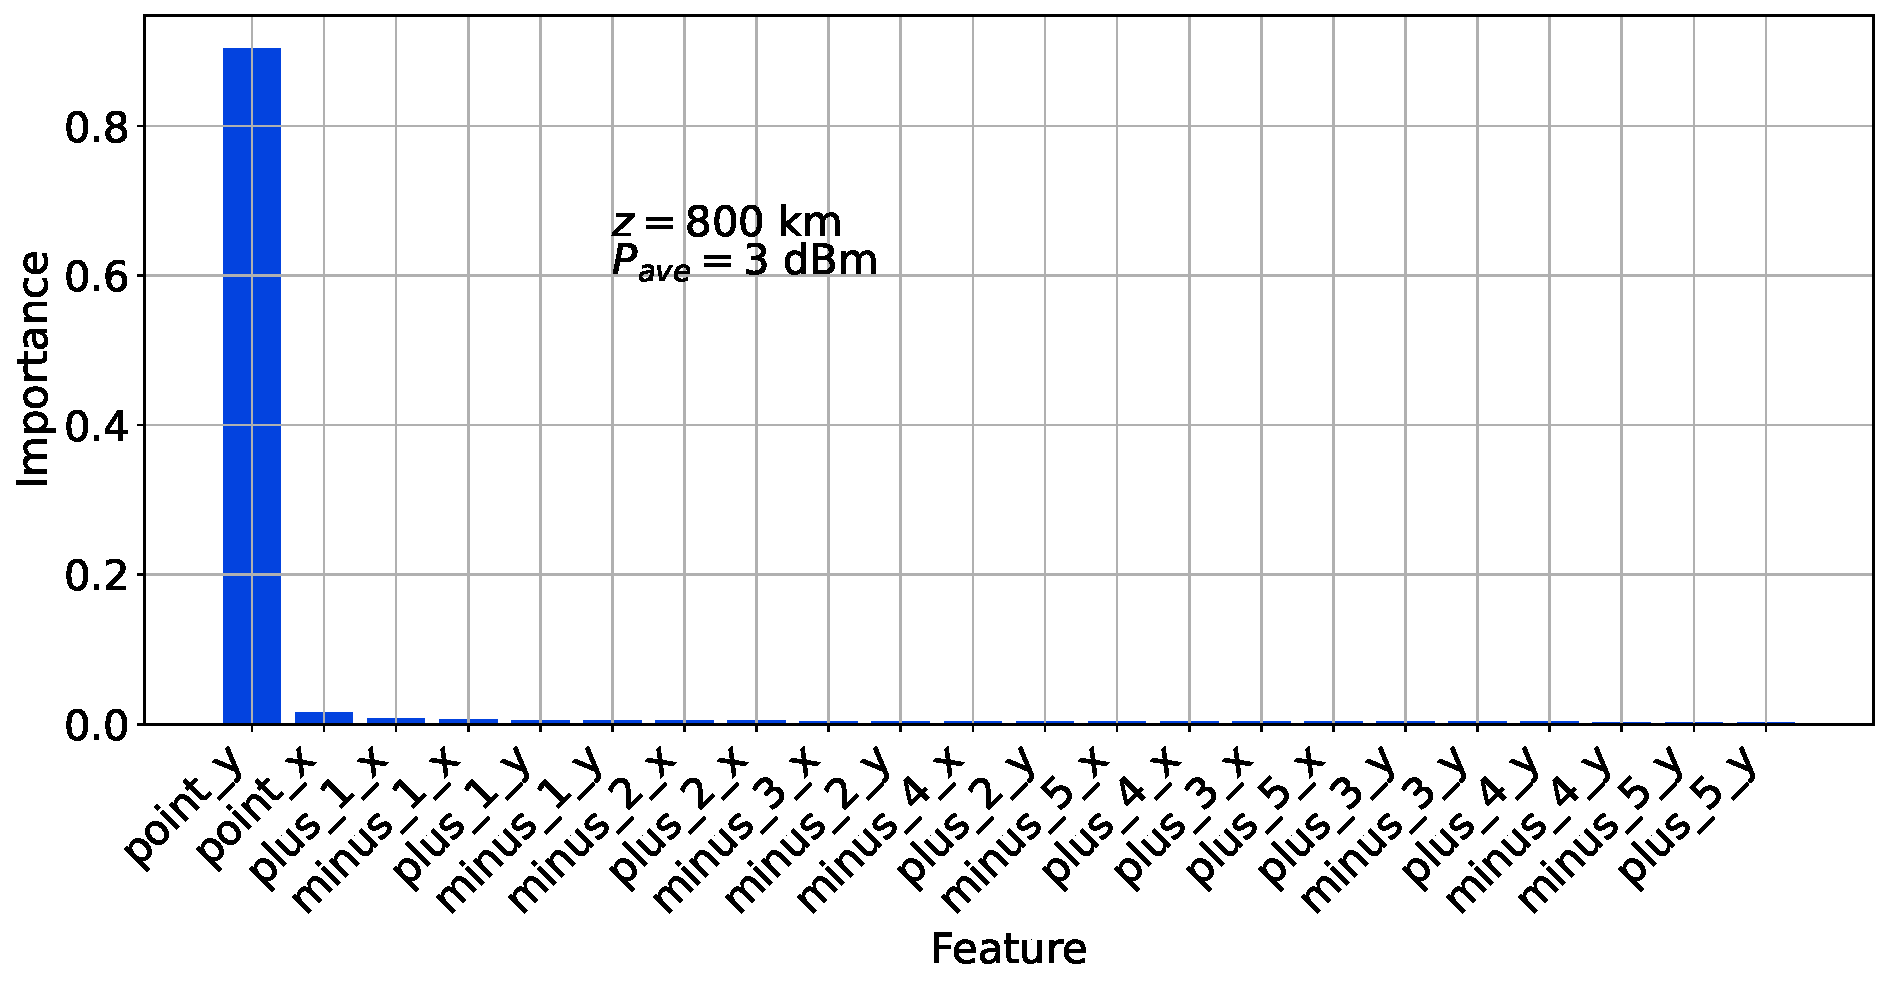
\includegraphics[width=1\linewidth]{images/boost/feature_importances_z800_pdbm3.pdf}
    }
    \end{minipage}

    \centering
    \begin{minipage}[h]{0.75\linewidth}
    \center{
        (b) 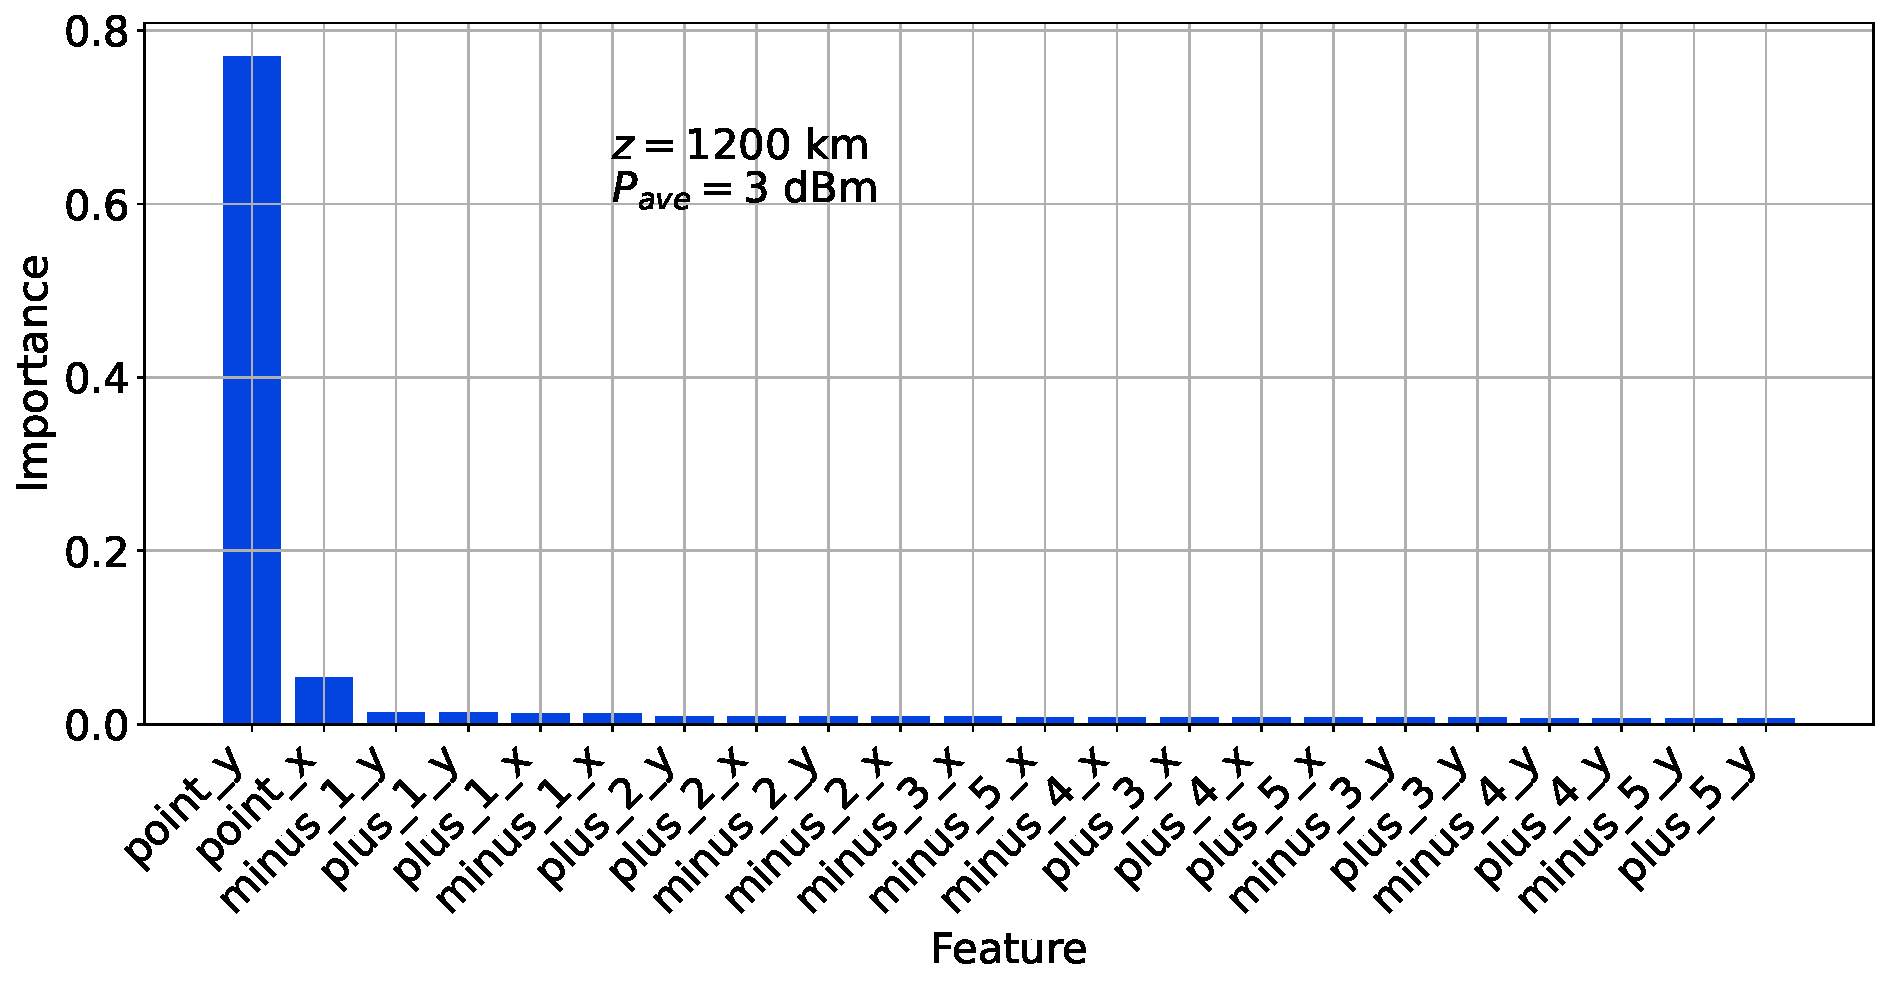
\includegraphics[width=1\linewidth]{images/boost/feature_importances_z1200_pdbm3.pdf}
    }
    \end{minipage}

    \centering
    \begin{minipage}[h]{0.75\linewidth}
    \center{
        (c) 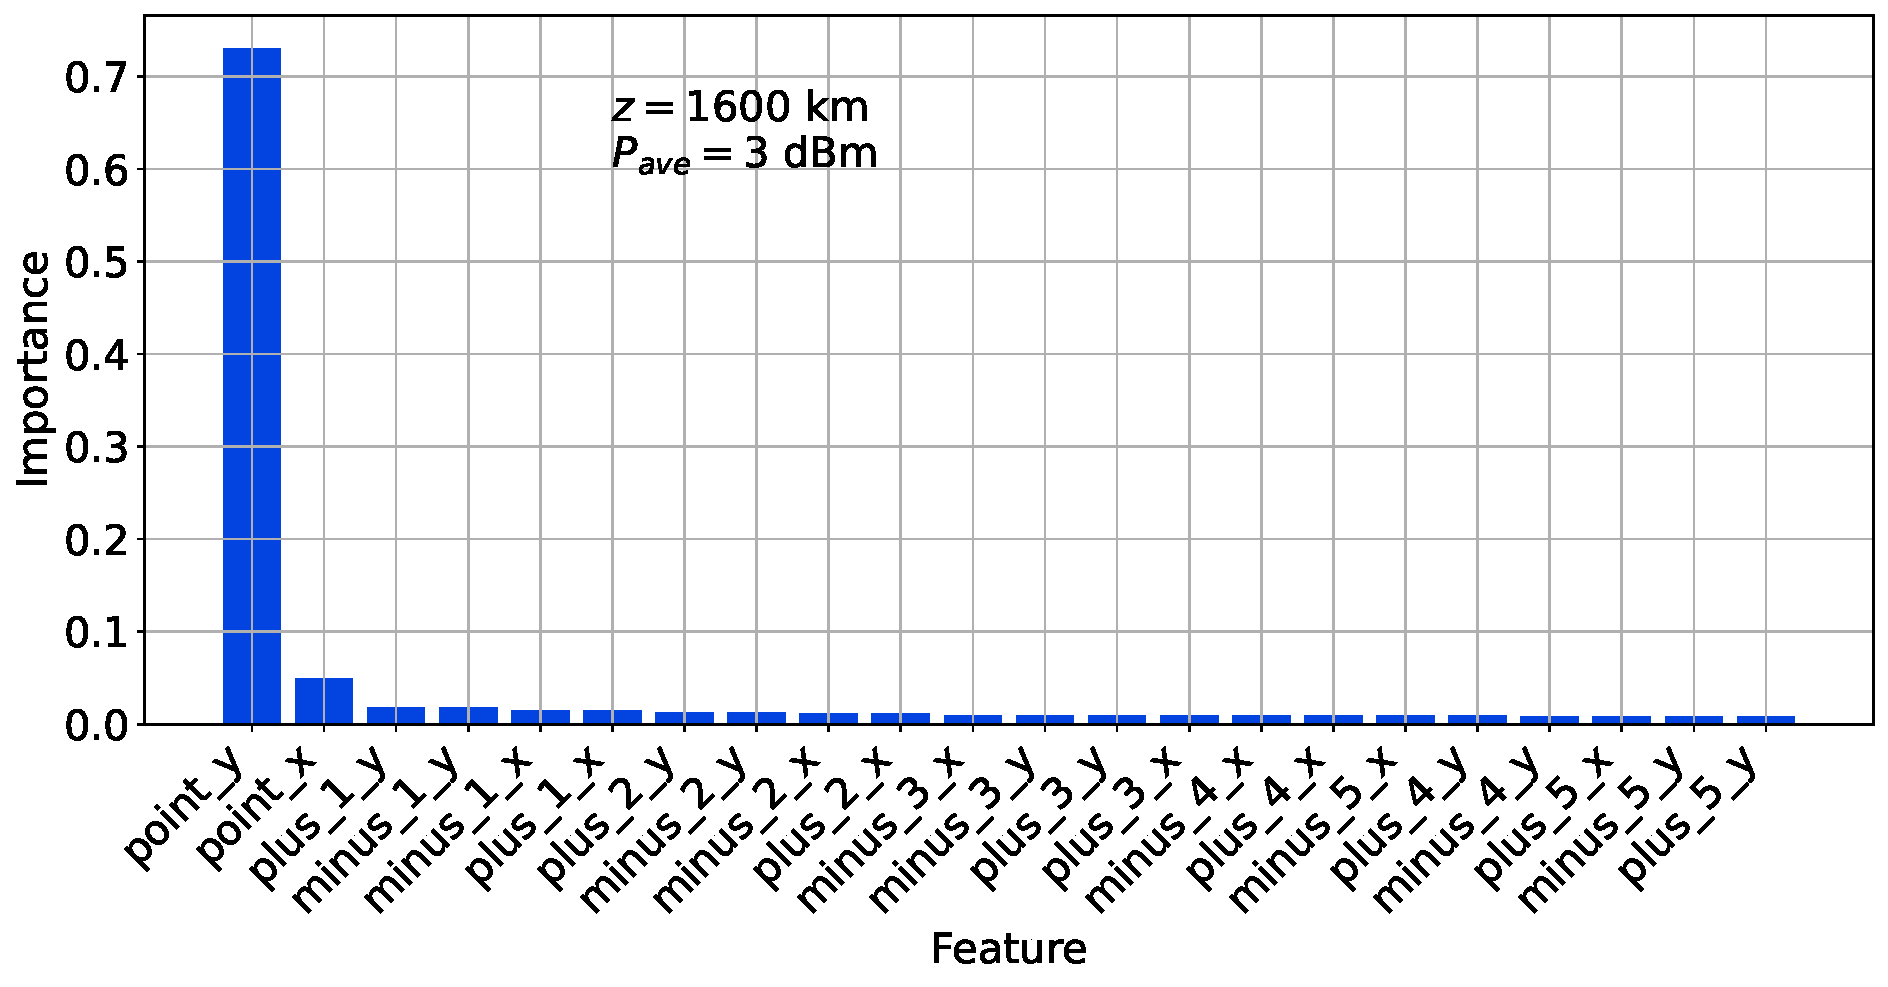
\includegraphics[width=1\linewidth]{images/boost/feature_importances_z1600_pdbm3.pdf}
    }
    \end{minipage}
    \caption{Feature importance in the trained \acrshort{gb} model for predicting nonlinear shifts at an average signal power of 3 dBm. \textbf{(a)} For a transmission distance of 800 km, \textbf{(b)} 1200 km, and \textbf{(c)} 1600 km. In the feature labels, `x' and `y' denote the polarization of the signal point, whereas `plus' and `minus' indicate the right and left neighbors in the symbol sequence, respectively.}
    \label{fig:importance_gb_3dbm}
\end{figure}

From these observations, we conclude that the impact of distant neighbors grows with increasing transmission distance, though not dramatically. Including more symbols could enhance model performance, but the improvement is minimal for short distances and potentially up to 8\% for longer distances under optimal conditions. This increase, while notable, does not fundamentally alter the model's overall performance. At a lower average signal power of 3 dBm, where nonlinear effects are reduced, the impact of distant neighbors is even less significant, reinforcing the dominant role of `point\_y' (Fig.~\ref{fig:importance_gb_3dbm}).

This analysis supports our methodological choice of focusing on five neighboring symbols, demonstrating its viability even when the actual channel memory extends significantly further. Our aim was to establish a proof of concept for using the \acrshort{gb} model without delving into a comprehensive study of neighbor influence, highlighting this as a promising direction for future research.

\subsection{Complexity}

\subsubsection{Constructing}
The computational complexity of constructing a decision tree depends on the number of records ($N$) and the number of features ($M$). In a balanced tree scenario, the complexity is $O(MN\log N)$, accounting for evaluating all features across all records at each level of the tree down to a depth of $\log N$.
In the worst-case, with an unbalanced tree structure, the complexity can escalate to $O(MN^2)$. This is due to the potential for the tree to degenerate into a structure with depth $N$, requiring extensive computations at each level.
Introducing a maximum depth limit ($D_{max}$) as a stopping criterion alters the complexity. Regardless of being balanced or unbalanced, the tree cannot exceed this depth, making the construction complexity $O(MND_{max})$. This constraint ensures that the tree's growth is curtailed, preventing the exponential increase in computational cost seen in unbounded scenarios.

The computational complexity of Decision Trees varies significantly between the ideal, balanced tree scenario and the worst-case, unbalanced tree. The introduction of a maximum tree depth as a stopping criterion significantly impacts the computational complexity of Decision Trees, both in construction and prediction phases. It provides a practical mechanism to control the growth of the tree, thereby ensuring that the complexity remains manageable, especially in scenarios that could otherwise lead to highly unbalanced structures.

In the context of \acrlong{gb}, the construction of the ensemble model involves sequentially building $T$ decision trees. Consequently, the computational complexity for training the ensemble is influenced by the complexities inherent in constructing individual decision trees, scaled by the number of trees, $T$. In scenarios where decision trees are balanced, the training complexity is $O(TMN\log N)$. Conversely, in cases where the trees become unbalanced, the computational burden escalates, with complexity potentially reaching $O(TMN^2)$. This increase is attributable to the deeper tree structures that may arise, requiring more extensive computation at each level. To mitigate such variability and enhance predictability in computational demands, imposing a maximum depth, $D$, for each tree normalizes the complexity to $O(TMND)$.

\subsubsection{Making Predictions}
For predictions, a balanced tree allows for traversing from the root to a leaf node in $O(\log N)$ computations, given the tree's depth corresponds to $\log N$ in balanced conditions.
In an unbalanced tree, the depth could approach $N$, leading to a worst-case prediction complexity of $O(N)$ for traversing through all nodes from root to a specific leaf.
When a maximum depth is enforced, the complexity of making a prediction becomes $O(D_{max})$. This limit ensures that the prediction time remains constant, relative to the depth constraint, regardless of the tree's balance.

Predictive complexity in \acrlong{gb} models similarly hinges on the depth of the individual decision trees. Under regular conditions, where trees maintain a balanced structure, the complexity of making predictions for a single instance is $O(T\log N)$, benefiting from the logarithmic depth of balanced trees. However, in the worst-case scenario, where trees may be significantly unbalanced, the complexity could deteriorate to $O(TN)$. To counteract this and secure a uniform prediction time, enforcing a maximum tree depth, $D$, aligns the predictive complexity to $O(TD)$.

The computational complexity for predictions made by the \acrlong{gb} algorithm can be succinctly summarized by the following upper limit:
\begin{equation}
    C(\mathrm{GB}) = T \cdot D,
\end{equation}
where \(T\) represents the number of trees within the \acrlong{gb} model, and \(D\) signifies the maximum depth encountered across all these trees. It's important to note that in practical applications, \(D\) does not typically surpass a threshold (often around 100). This constraint helps in managing the computational load during the prediction phase, ensuring that the time complexity remains within a feasible range, even as the model scales.

This formulation emphasizes the linear relationship between the algorithm's computational complexity and both the number of trees and their depth. Such an understanding is crucial for optimizing the performance and efficiency of \acrlong{gb} models in diverse applications.
At first glance, it may appear that the overall complexity for our chosen set of parameters is excessively high. In this study, our primary goal is not to achieve cutting-edge complexity but rather to demonstrate the proof-of-concept. However, it is important to emphasize that each parameter contributing to complexity can be optimized to significantly reduce the overall complexity. Comprehensive information about feature importance allows us to manage input parameters (which can be further reduced) and to control the impact of each decision tree, thereby enabling the removal of unnecessary trees to enhance performance. Moreover, we can manually regulate the maximum depth of each tree, which, after optimization, can ultimately yield the desired performance.

% The complexity of prediction for gradient boosting can be expressed using the following formula:
% $$
% C(GB) = N_{trees} \cdot M \cdot N_{features}
% $$
% where $C(GB)$ represents the complexity of prediction for gradient boosting, $N_{trees}$ is the number of trees in the ensemble, $M$ is the maximum depth of each tree, $N_{features}$ is the number of features in the dataset.

% This formula assumes that the complexity of each decision in the tree is constant and that the trees have a balanced structure. In practice, the trees might not be perfectly balanced, and the actual complexity could be somewhat lower. However, this formula provides a useful estimate for understanding the relationship between the main parameters of gradient boosting and its prediction complexity.




\subsection{Results}

\begin{figure}[ht]
    \begin{minipage}[h]{0.49\linewidth}
    \center{
        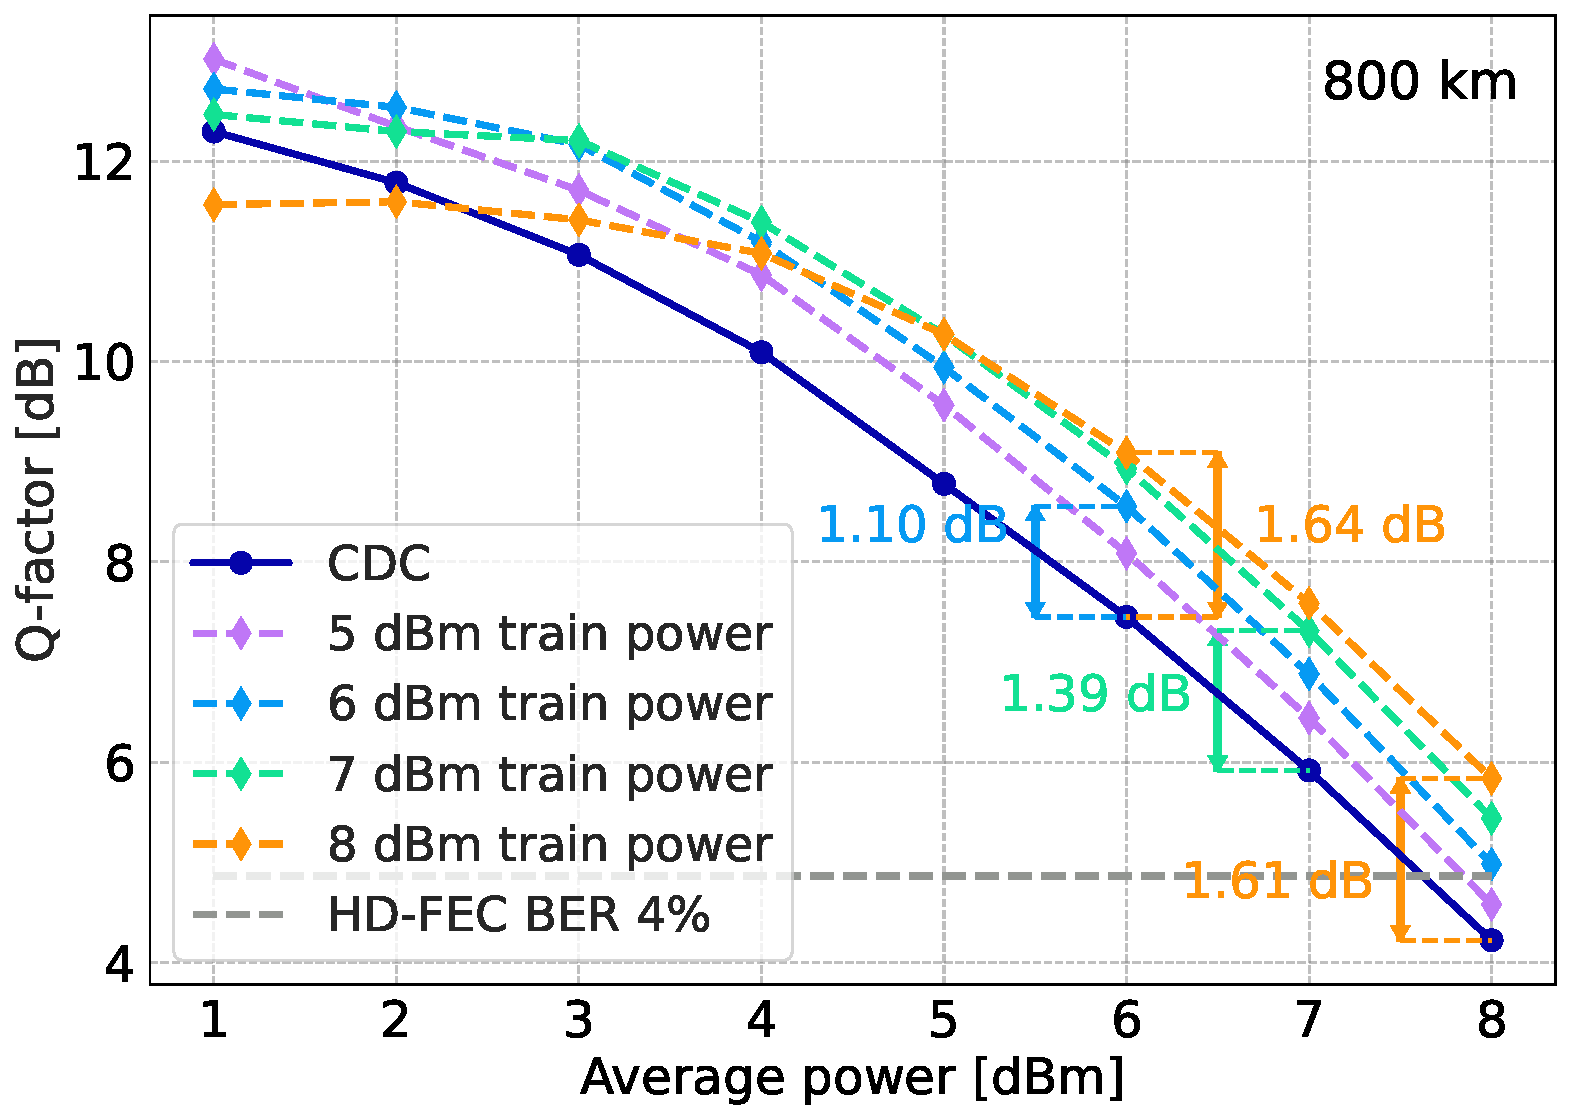
\includegraphics[width=1\linewidth]{images/boost/q_different_models_single_800.pdf} (a) \\
    }
    \end{minipage}
    \hfill
    \begin{minipage}[h]{0.49\linewidth}
    \center{
        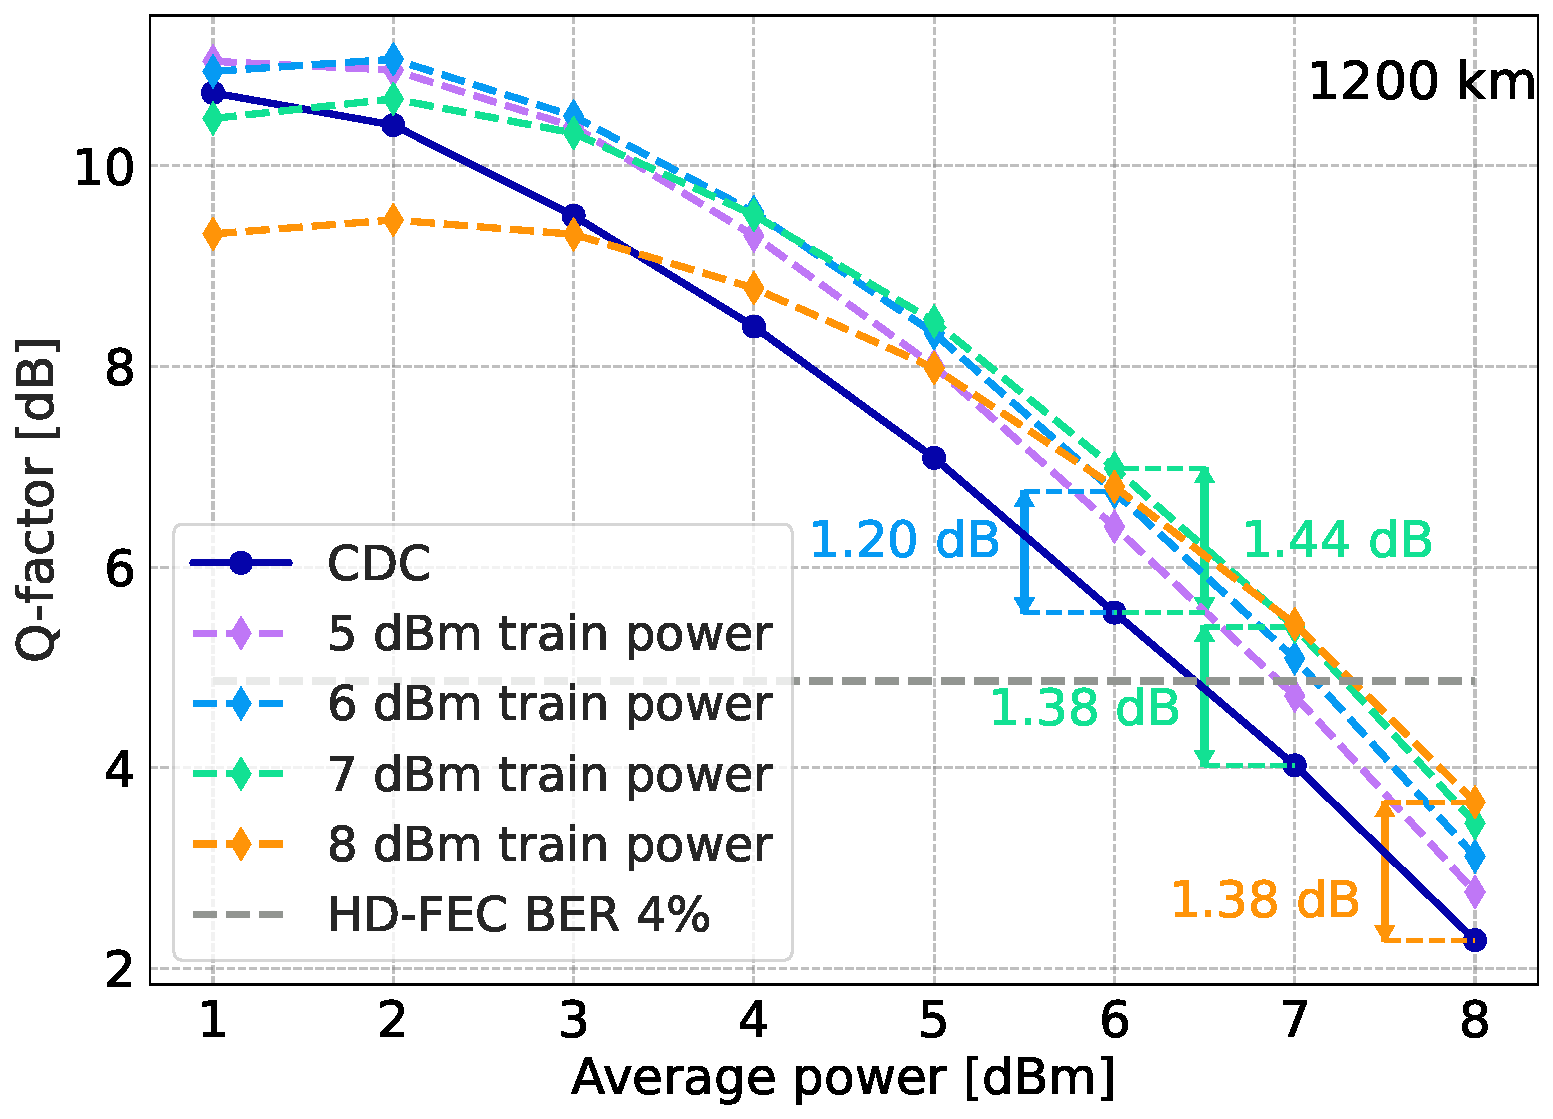
\includegraphics[width=1\linewidth]{images/boost/q_different_models_single_1200.pdf} (b) \\
    }
    \end{minipage}
    \vfill
    \center{
        \begin{minipage}[h]{0.49\linewidth}
        \center{
            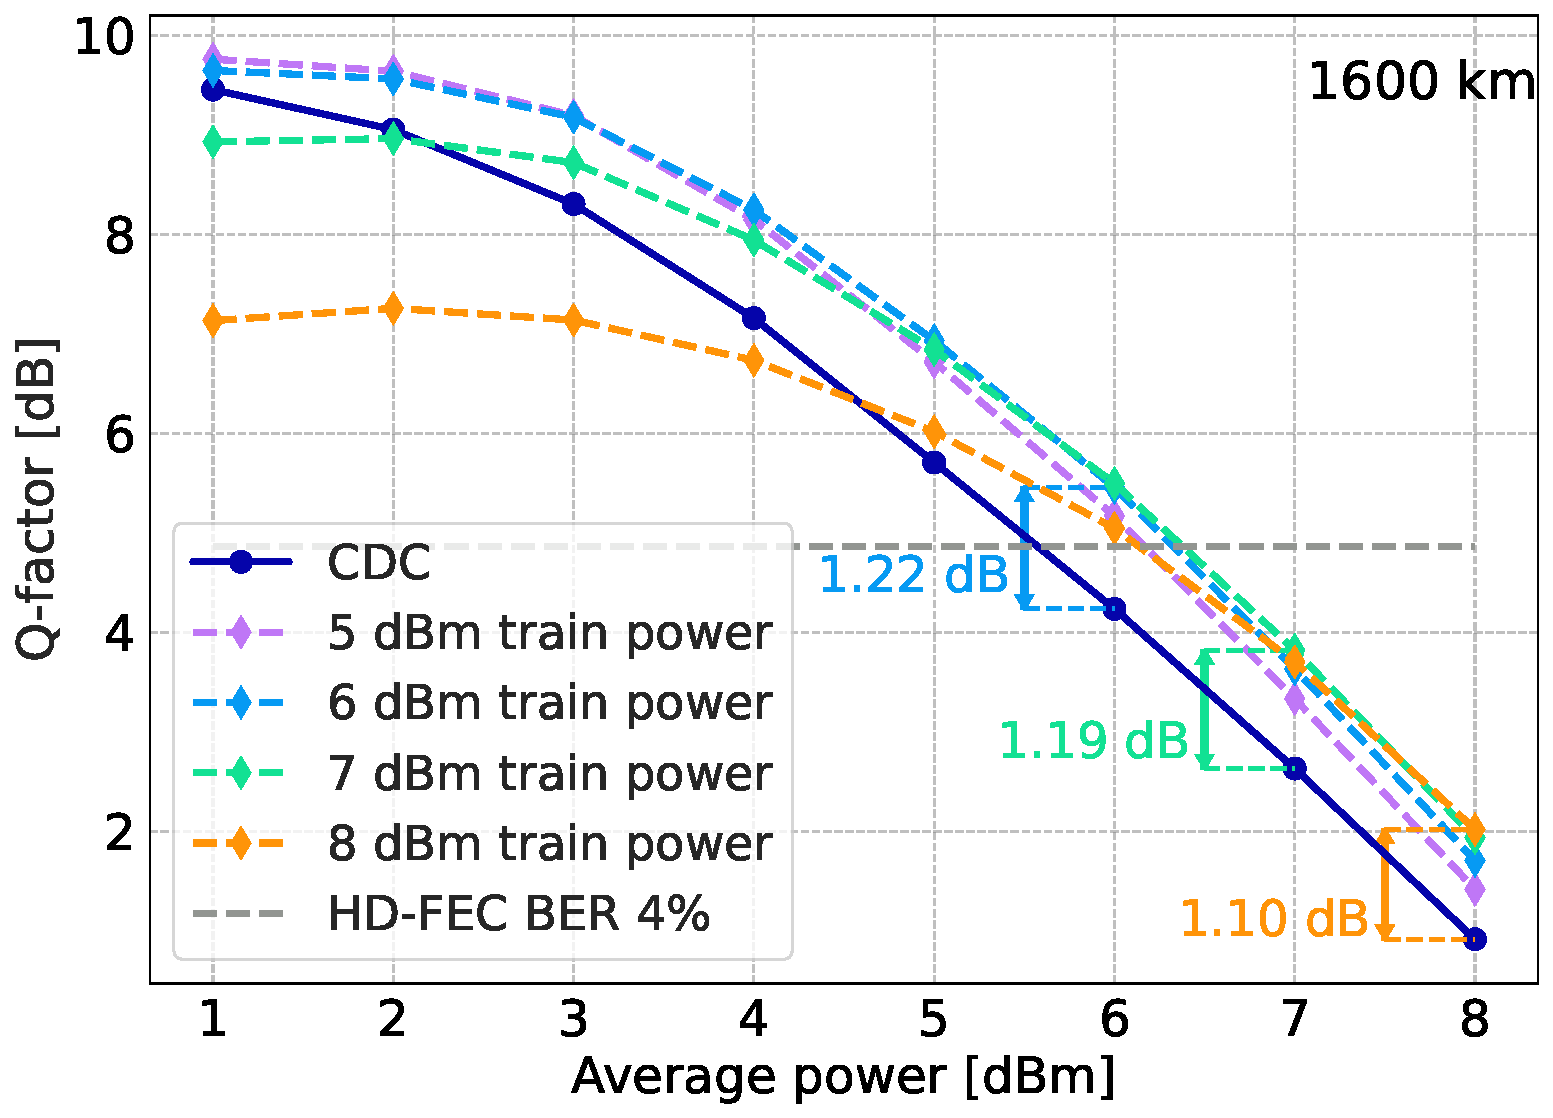
\includegraphics[width=1\linewidth]{images/boost/q_different_models_single_1600.pdf} (c) \\
        }
        \end{minipage}
    }
    \caption{Q-Factor performance after nonlinear equalization using \acrshort{gb} trained at varying average signal power levels. Solid lines represent the system with CDC, and horizontal dashed lines indicate the HD-FEC threshold for a \acrshort{ber} of 4\%. Total propagation distance of 800 km \textbf{(a)}, 1200 km \textbf{(b)} and 1600 km \textbf{(c)}.}
    \label{fig:boost_result}
\end{figure}


% \begin{figure*}[ht]
%    \centering
%     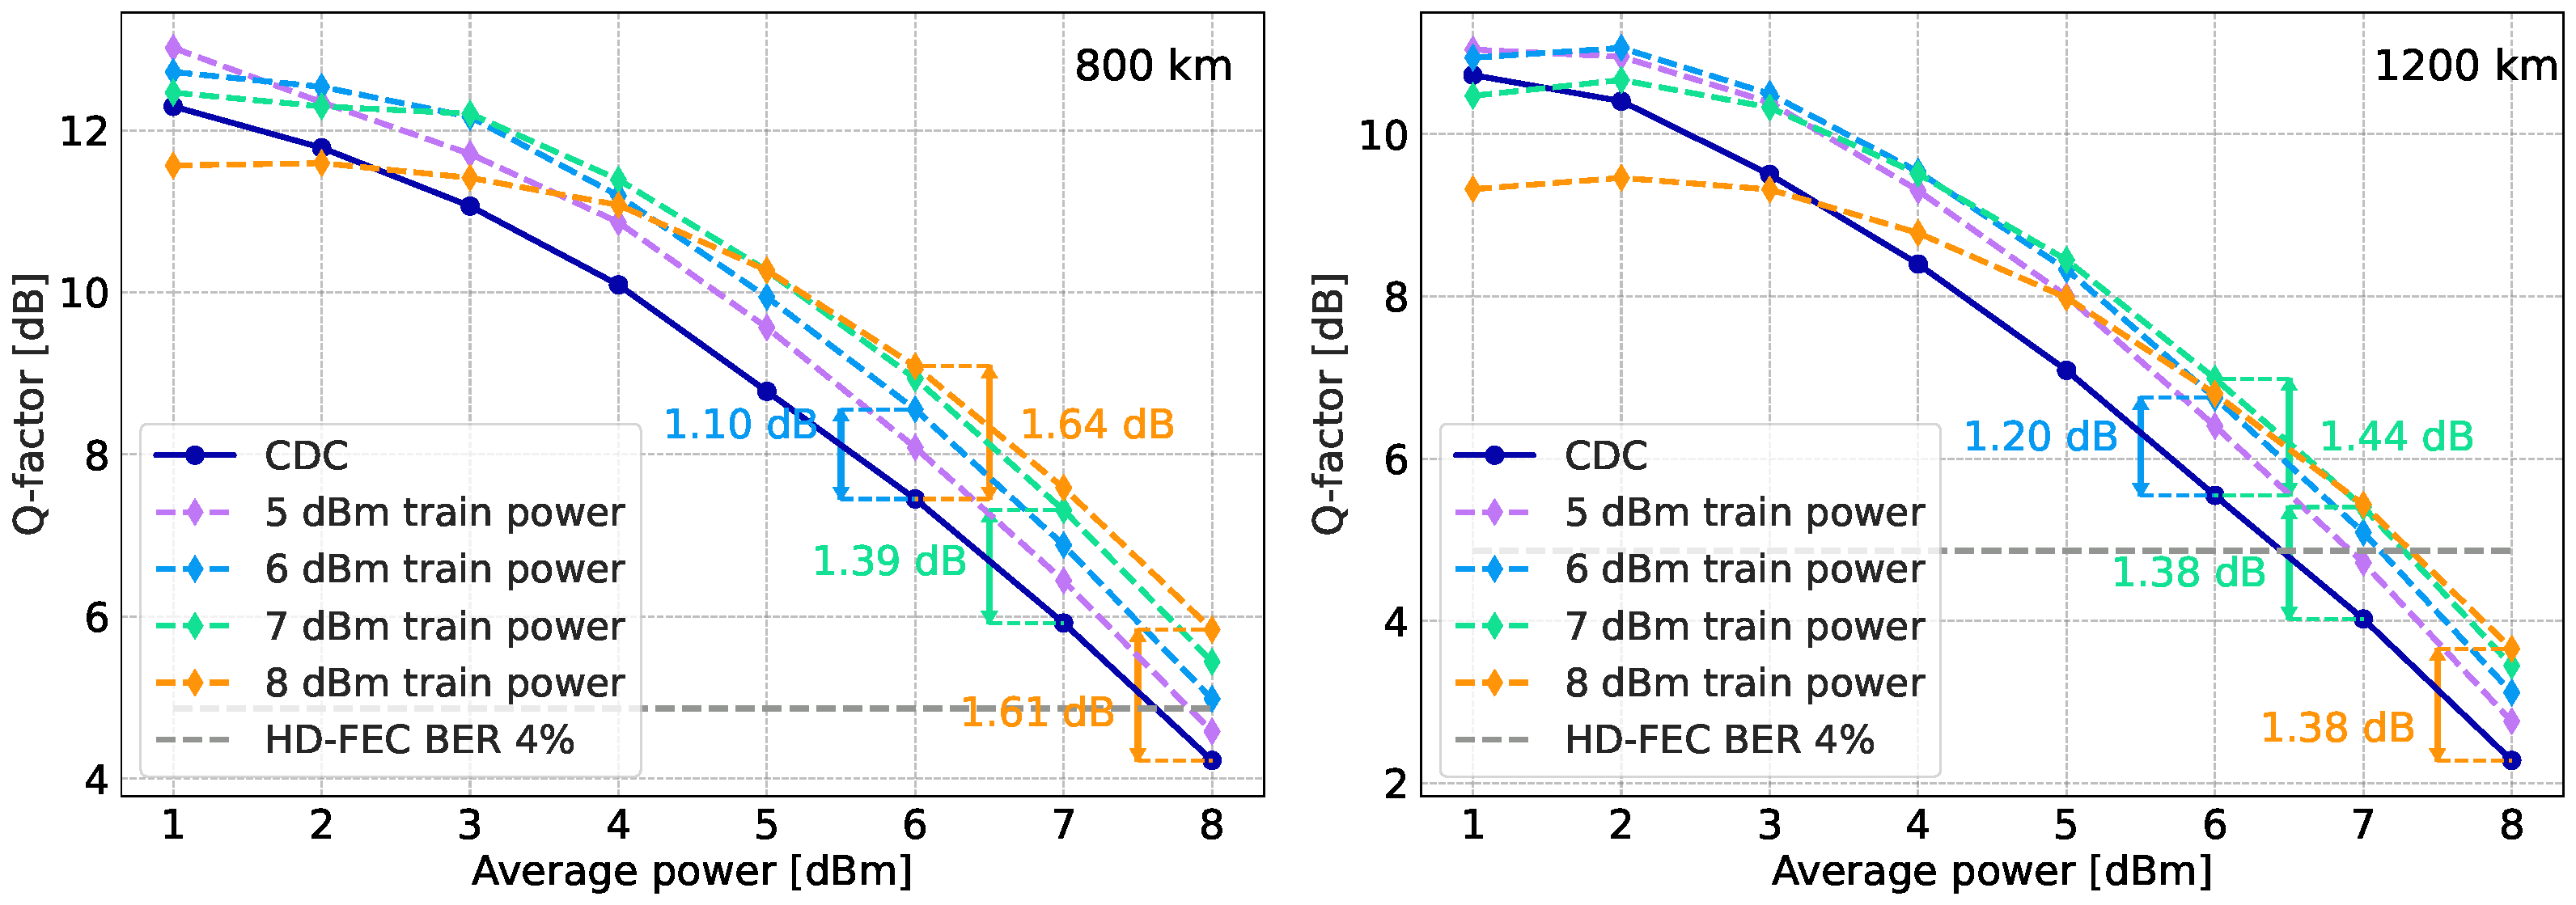
\includegraphics[width=1\linewidth]{images/boost/q_different_models_couple.pdf}
%     \caption{Q-Factor performance after nonlinear equalization using GB trained at varying average signal power levels. Solid lines represent the system with CDC, and horizontal dashed lines indicate the HD-FEC threshold for a BER of 4\%. Total propagation distance of 800 km \textbf{(left)}, and 1200 km \textbf{(right)}.}
%     \label{fig:fig1}
% \end{figure*}

% \begin{figure}[ht]
%    \centering
%         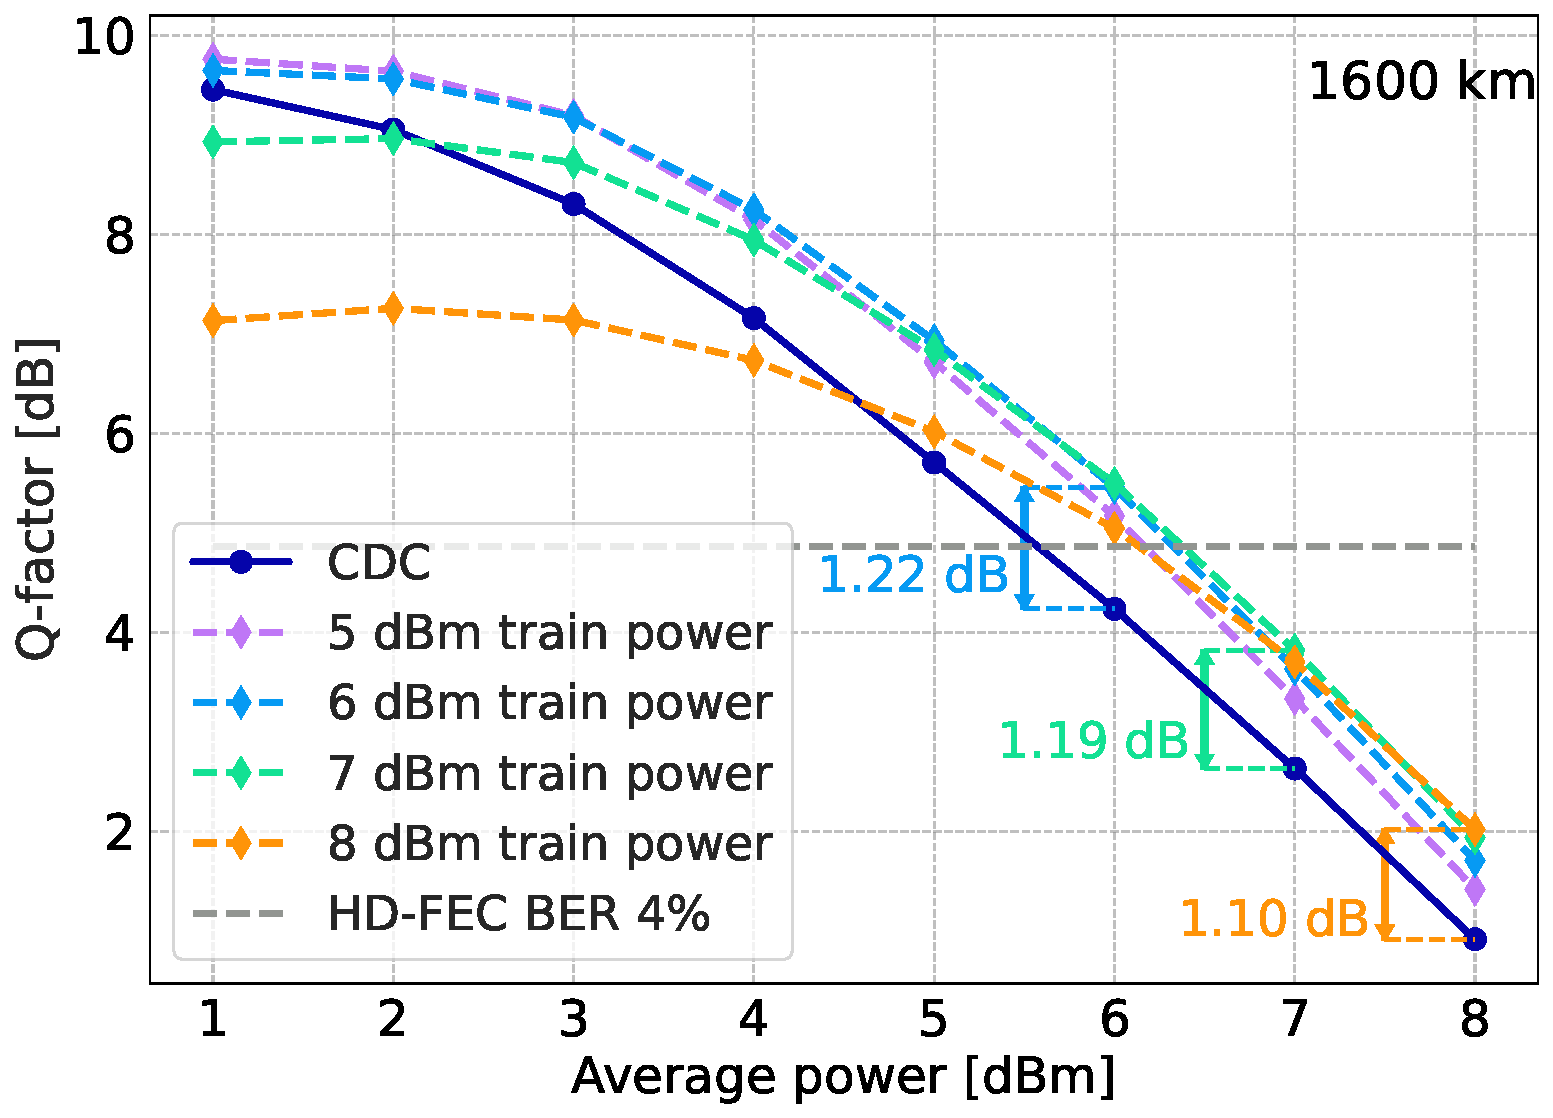
\includegraphics[width=0.5\linewidth]{images/boost/q_different_models_single.pdf}
%     \caption{Analogous to Fig.~\ref{fig:fig1}, Q-Factor performance for a total propagation distance of 1600 km, after nonlinear equalization using GB trained at different average signal power levels.}
%     \label{fig:fig2}
% \end{figure}


To demonstrate the potential of \acrshort{gb}, we assessed the performance of various \acrshort{gb} models across a range of propagation distances and diverse input signal average powers. The results were analyzed in terms of Q-factor improvement and the level of HD-FEC (Hard Decision Forward Error Correction), which represents a common error correction scheme used in optical communication systems. The target \acrlong{ber} was set at $4\%$.

For all propagation distances, the \acrshort{gb} models showed at least a $1\;\textrm{dB}$ improvement in Q-factor compared to the system with Chromatic Dispersion Compensation (CDC). Specifically, for a $1600\;\textrm{km}$ transmission distance (Fig.~\ref{fig:boost_result}c), the model trained on $8\;\textrm{dBm}$ signals exhibited a $1.10\;\textrm{dB}$ improvement in Q-factor for the same test power. The model trained on $7\;\textrm{dBm}$ signals displayed a $1.19\;\textrm{dB}$ improvement for the same test power, while the model trained on $6\;\textrm{dBm}$ signals showed a $1.22\;\textrm{dB}$ improvement. The $1.22\;\textrm{dB}$ Q-factor improvement for the $6\;\textrm{dBm}$ model allowed us to decrease the \acrshort{ber} (increase the Q-factor) below (above) the HD-FEC level.

Interestingly, models trained on higher average power (and thus experiencing higher nonlinear distortions) exhibited good performance when applied to lower test power levels. However, their performance degraded for higher test power levels. This observation suggests that the \acrshort{gb} algorithm can successfully mitigate nonlinear effects. This is particularly evident in Fig.~\ref{fig:boost_result}a for a propagation distance of $800\;\textrm{km}$. The model trained on $8\;\textrm{dBm}$ outperformed other models for power levels from $5\;\textrm{dBm}$ to $8\;\textrm{dBm}$, showing approximately $1.6\;\textrm{dB}$ improvement (specifically, $1.64\;\textrm{dB}$ for $6\;\textrm{dBm}$ test power and $1.61\;\textrm{dB}$ for $8\;\textrm{dBm}$ test power). For $8\;\textrm{dBm}$, the improved Q-factor surpassed the HD-FEC level. However, for lower signal powers, the model trained on $8\;\textrm{dBm}$ performed poorly, since these regimes are less influenced by nonlinear effects.

A similar pattern can be observed in Fig.~\ref{fig:boost_result}b for a propagation distance of $1200\;\textrm{km}$. In this case, the model trained on $7\;\textrm{dBm}$ showed significant improvement for a wide range of test signal powers (from $3\;\textrm{dBm}$ to $8\;\textrm{dBm}$). This finding indicates that the \acrshort{gb} training power can be optimized for specific power ranges in which the system operates. The wide range of applicability allows for the development of a universal equalizer based on \acrshort{gb}, which does not require retraining for different power levels (subject to the constraints of the working regime for \acrshort{gb}).


\subsection{Discussion}
\subsubsection{Perspective of Practical Realization}

To address the practical aspects of signal equalization, it is crucial to consider the computational efficiency of the equalization process in real-world implementations. \acrlong{nn}s (\acrshort{nn}s), for instance, comprise multiple layers involving matrix multiplications, typically resulting in computational complexity on the order of $O(N^3)$ for straightforward implementations. While optimizations such as Strassen's algorithm can reduce this complexity, the inherent structure of neural networks, often comprising several layers, significantly increases the operation count, scaling almost cubically with added complexity. This escalation can range from thousands of operations for basic \acrfull{mlp} architectures to millions for more sophisticated models, which offer improved performance but at a higher computational cost.

The sequential nature of these operations, a characteristic shared with \acrfull{dbp} algorithms employing the \acrfull{ssfm}, necessitates waiting for the completion of previous operations before proceeding. This requirement for shared memory, where the results of prior computations must be immediately accessible for subsequent operations, introduces significant challenges for real-time processing.

The \acrlong{gb} approach offers a noteworthy advancement in this context. Once the estimators, or trees, are constructed, they can be utilized independently. This independence allows for the parallel computation of results from each tree without interdependencies, significantly enhancing computational efficiency. Furthermore, the simplicity of \acrshort{gb} operations—requiring only $D$ (the depth of the tree) comparisons for input features to derive results from each decision tree—eliminates the need for complex computations. Given that comparison operations are as fast as summations in contemporary systems, the process is highly efficient. Importantly, the depth of these trees, $D$, is inherently manageable, often not exceeding 20 in practical analyses.

With only 20 basic operations, we can process all trees in a \acrlong{gb} model. This efficiency suggests the potential for high-speed performance through parallel processing. An intriguing research direction is exploring how to manage 200,000 estimators, the current count in our system, in parallel within real-world platforms like \acrshort{fpga}s. Furthermore, there's room to optimize and potentially reduce this number of estimators, which hints at the depth of investigation required --- a fitting challenge for a dedicated Ph.D. project. In this thesis, my aim was to establish a proof-of-concept for the \acrshort{gb} algorithm, demonstrating its viability.

\subsubsection{Conclusion}
% In conclusion, this study has demonstrated the potential of gradient boosting as a novel equalization technique in optical communication systems, offering better predictive performance with the possibility of reduced complexity compared to traditional methods. This innovative approach may pave the way for advancements in the field and enhance the efficiency of modern telecommunication networks.

% Future research should focus on optimizing the complexity-performance trade-off, investigating real-world robustness, and exploring hardware acceleration opportunities. Developing a universal equalizer based on gradient boosting could further expand the applicability of this technique in optical communication systems.

In conclusion, this study highlights the potential of gradient boosting as an innovative equalization technique in optical communication systems. This approach not only offers improved predictive performance but also holds the promise of simplifying the complexity inherent in traditional methods. Such advancements could significantly enhance the efficiency of contemporary telecommunication networks. 

Our initial findings are encouraging, showing that models based on gradient boosting can achieve a notable improvement in system performance, specifically an increase of 1.1 - 1.6 dB in the Q-factor compared to systems that only implement \acrfull{cdc}. This underscores both the practical and theoretical value of the gradient boosting technique in advancing optical communication technologies.

Looking forward, future research should aim at fine-tuning the balance between complexity and performance, ensuring robustness in real-world applications, and examining the prospects of hardware acceleration to bring this technique to practical use. The development of a versatile equalizer using gradient boosting could broaden the scope of its application in optical communications, promising substantial improvements in the field.
